%\documentclass[final,authoryear,1p]{elsarticle}
%\documentclass[final,authoryear,5p,times,twocolumn]{elsarticle}
%\documentclass[authoryear,preprint,review,9pt]{elsarticle}
\documentclass[journal]{IEEEtran}
\usepackage{amssymb}
\usepackage{amsmath}
\usepackage{bbm}
\usepackage{graphicx}
\usepackage{subfig}
\usepackage{algorithmic}
\usepackage{algorithm}
\usepackage{relsize}
\usepackage{booktabs}
\usepackage{color}
\usepackage[labelfont={small,bf}]{caption}
\usepackage[font={small,bf}]{caption}
\usepackage[numbers]{natbib}
\renewcommand{\bibfont}{\footnotesize}
\usepackage[margin=0.6in]{geometry}
\newcommand{\closer}{\vspace{-0.0cm}}
\newcommand{\figcloser}{\vspace{-0.4cm}}

\begin{document}

\title{\Large Symmetric Diffeomorphic Registration with \\ Expected Cross-Correlation for Multi-Modal Brain MRI\\ {\large Supplementary material}}
\author{
    \IEEEauthorblockN{{\bf Omar Ocegueda}}~\and~
    \IEEEauthorblockN{{\bf Eleftherios Garyfallidis}}~\and~
    \IEEEauthorblockN{{\bf Maxime Descoteaux}}~\and~
    \IEEEauthorblockN{{\bf Mariano Rivera}}\\
}

\maketitle
\section{Semi-synthetic image construction}
Video ``$semi\_synthetic.mp4$'' illustrates the procedure to generate the semi-synthetic images from the Brainweb template and the real, annotated, T1 brain images. Note that, the more accurate the registration, the more realistic the constructed image is.\\

\section{Detailed quantitative results}

We first present the average Jaccard indices of tissue types: White Matter (WM), Gray Matter (GM) and Cerebrospinal Fluid (CSF) instead of localized anatomical areas. Although overlap of tissue types may not be a good indicator of registration performance in general \cite{Rohlfing2012} (overlap of localized anatomical regions is preferred), it still provides insights on what method is expected to perform better for registration-based segmentation, which may be used to define anatomical priors to improve tractography \cite{Smith2012, Girard2014}. Table \ref{tab:monomodal_results_segTri_fill} shows the results in the mono-modal case, and Table \ref{tab:multimodal_results_segTri_fill} shows the corresponding results in the multi-modal case (T1 - T2).
% Table generated by Excel2LaTeX from sheet 'SyNEM-Monomodal-Large'
\begin{table}[htbp]
  \centering
  {\small
    \begin{tabular}{rrrr}
    \toprule
    \textbf{} & \textbf{SyN-EM} & \textbf{SyN-ECC} & \textbf{SyN-CC} \\
    \midrule
    \textbf{Background} & 0.994 & 0.995 & \textbf{0.995} \\
    \textbf{CSF} & 0.335 & 0.349 & \textbf{0.359} \\
    \textbf{Gray Matter} & 0.740 & \textbf{0.765} & 0.759 \\
    \textbf{White Matter} & 0.703 & \textbf{0.739} & 0.728 \\
    \bottomrule
    \end{tabular}%
    \caption{Comparison of the registration performance (measured by the Jaccard index over Background, CSF, GM and WM)of the Greedy SyN algorithm with EM, ECC and CC metrics. The Jaccard
indices were averaged over 306 monomodal registrations. Top performer for each region is highlighted.}
  \label{tab:monomodal_results_segTri_fill}}%
\end{table}%

% Table generated by Excel2LaTeX from sheet 'SyNEM-Multi-Large'
\begin{table}[htbp]
  \centering
  {\small
    \begin{tabular}{ccccc}
    \toprule
          & \textbf{SyN-EM} & \textbf{SyN-ECC} & \textbf{SyN-CC} & \textbf{SyN-MI} \\
    \midrule
    \textbf{Background} & 0.993 & 0.995 & 0.990 & \textbf{0.995} \\
    \textbf{CSF} & 0.275 & \textbf{0.335} & 0.157 & 0.325 \\
    \textbf{Gray Matter} & 0.718 & \textbf{0.742} & 0.597 & 0.691 \\
    \textbf{White Matter} & 0.685 & \textbf{0.718} & 0.572 & 0.622 \\
    \bottomrule
    \end{tabular}}%
  \caption{Comparison of the registration performance (measured by the Jaccard index over Background, CSF, GM and WM)of the Greedy SyN algorithm with EM, ECC, CC and MI metrics.
The Jaccard indices were averaged over 612 multimodal registrations. Top performer for each region is highlighted.}
  \label{tab:multimodal_results_segTri_fill}%
\end{table}%

% Table generated by Excel2LaTeX from sheet 'SyNEM-Monomodal-Large'
\begin{table}[p]
\begin{adjustwidth}{-0.75cm}{}
  {\centering
    \small
    \begin{tabular}{lcccc}
    \toprule
    \textbf{}& \textbf{SyN-EM} & \textbf{SyN-ECC} & \textbf{SyN-CC} & \textbf{SyN-MI} \\
    \midrule
    \textbf{Brain-Stem} & 0.786 & \textbf{0.816} & 0.812 & 0.804 \\
    \textbf{Right-Cerebellum-Cortex} & 0.736 & \textbf{0.815} & 0.813 & 0.771 \\
    \textbf{Left-Cerebellum-Cortex} & 0.739 & \textbf{0.811} & 0.808 & 0.766 \\
    \textbf{Right-Thalamus-Proper} & 0.714 & 0.766 & \textbf{0.772} & 0.745 \\
    \textbf{Left-Thalamus-Proper} & 0.727 & 0.763 & \textbf{0.767} & 0.748 \\
    \textbf{Right-Putamen} & 0.681 & 0.748 & \textbf{0.751} & 0.712 \\
    \textbf{Left-Putamen} & 0.699 & 0.744 & \textbf{0.744} & 0.721 \\
    \textbf{Left-Cerebral-Cortex} & 0.724 & \textbf{0.739} & 0.733 & 0.687 \\
    \textbf{Right-Cerebral-Cortex} & 0.719 & \textbf{0.739} & 0.731 & 0.683 \\
    \textbf{Right-Cerebral-White-Matter} & 0.702 & \textbf{0.733} & 0.720 & 0.645 \\
    \textbf{Left-Cerebral-White-Matter} & 0.705 & \textbf{0.732} & 0.721 & 0.646 \\
    \textbf{Left-Lateral-Ventricle} & 0.731 & 0.727 & \textbf{0.732} & 0.718 \\
    \textbf{Right-Lateral-Ventricle} & 0.709 & 0.714 & \textbf{0.717} & 0.699 \\
    \textbf{Right-Cerebellum-White-Matter} & 0.576 & \textbf{0.701} & 0.691 & 0.608 \\
    \textbf{Left-Cerebellum-White-Matter} & 0.581 & \textbf{0.701} & 0.693 & 0.611 \\
    \textbf{Left-Caudate} & 0.645 & \textbf{0.671} & 0.665 & 0.666 \\
    \textbf{Right-Caudate} & 0.620 & \textbf{0.655} & 0.647 & 0.651 \\
    \textbf{Right-VentralDC} & 0.612 & 0.651 & \textbf{0.652} & 0.628 \\
    \textbf{Left-VentralDC} & 0.622 & \textbf{0.651} & 0.650 & 0.631 \\
    \textbf{Right-Pallidum} & 0.498 & \textbf{0.622} & 0.620 & 0.582 \\
    \textbf{Right-Hippocampus} & 0.572 & \textbf{0.621} & 0.620 & 0.575 \\
    \textbf{Left-Pallidum} & 0.524 & \textbf{0.615} & 0.614 & 0.583 \\
    \textbf{Left-Hippocampus} & 0.574 & \textbf{0.610} & 0.609 & 0.564 \\
    \textbf{4th-Ventricle} & 0.551 & 0.606 & \textbf{0.608} & 0.574 \\
    \textbf{3rd-Ventricle} & 0.527 & 0.544 & \textbf{0.547} & 0.515 \\
    \textbf{Left-Amygdala} & 0.444 & 0.519 & \textbf{0.519} & 0.484 \\
    \textbf{Right-Amygdala} & 0.411 & 0.513 & \textbf{0.514} & 0.458 \\
    \textbf{Left-Accumbens-area} & 0.451 & 0.500 & \textbf{0.500} & 0.462 \\
    \textbf{Right-Accumbens-area} & 0.433 & 0.490 & \textbf{0.490} & 0.443 \\
    \textbf{Right-Inf-Lat-Vent} & 0.177 & 0.230 & \textbf{0.232} & 0.162 \\
    \textbf{Left-Inf-Lat-Vent} & 0.190 & 0.228 & \textbf{0.233} & 0.167 \\
    \hline
    \textbf{Average (std.)} & 0.593 (0.148) & 0.644 (0.142) & 0.643 (0.140) & 0.603 (0.149) \\
    \textbf{Rank-1 count} & 0 & 16 & 15 & 0 \\
    \textbf{Rank-2 count} & 1 & 14 & 14 & 2 \\
    \textbf{Rank-3 count} & 9 & 1 & 2 & 19 \\
    \bottomrule
    \end{tabular}}%
    \caption{Comparison of the registration performance (measured by the Jaccard index over 31 anatomical regions) of the Greedy SyN algorithm with EM, ECC, CC and MI metrics.
The Jaccard indices were averaged over 306 monomodal registrations. Rank-$k$ counts show the number of anatomical regions for which each
method ranked $k$ among the four methods under comparison. Top performer (rank-1) for each region is highlighted. }
  \label{tab:monomodal_results_seg}%
\end{adjustwidth}
\end{table}%

% Table generated by Excel2LaTeX from sheet 'SyNEM-Multi-Large'
\begin{table}[htbp]
  \centering
  {\small
    \begin{tabular}{rrrr}
    \toprule
          & \textbf{SyN-ECC} & \textbf{SyN-EM} & \textbf{SyN-CC} \\
    \midrule
    \textbf{Right-Thalamus-Proper:} & \textbf{0.758} & 0.716 & 0.756 \\
    \textbf{Left-Thalamus-Proper:} & \textbf{0.754} & 0.727 & 0.752 \\
    \textbf{Left-Lateral-Ventricle:} & 0.709 & 0.706 & \textbf{0.733} \\
    \textbf{Right-Lateral-Ventricle:} & 0.696 & 0.687 & \textbf{0.718} \\
    \textbf{Left-Putamen:} & \textbf{0.740} & 0.699 & 0.683 \\
    \textbf{Right-Putamen:} & \textbf{0.742} & 0.684 & 0.676 \\
    \textbf{Brain-Stem:} & \textbf{0.790} & 0.786 & 0.663 \\
    \textbf{Left-Cerebellum-Cortex:} & \textbf{0.765} & 0.729 & 0.649 \\
    \textbf{Right-Cerebellum-Cortex:} & \textbf{0.769} & 0.729 & 0.645 \\
    \textbf{Left-Caudate:} & \textbf{0.652} & 0.628 & 0.637 \\
    \textbf{Right-Caudate:} & \textbf{0.636} & 0.606 & 0.618 \\
    \textbf{Right-Cerebral-White-Matter:} & \textbf{0.723} & 0.683 & 0.571 \\
    \textbf{Left-Cerebral-White-Matter:} & \textbf{0.722} & 0.685 & 0.570 \\
    \textbf{Left-Cerebral-Cortex:} & \textbf{0.700} & 0.699 & 0.558 \\
    \textbf{Right-Cerebral-Cortex:} & \textbf{0.697} & 0.694 & 0.548 \\
    \textbf{4th-Ventricle:} & \textbf{0.583} & 0.546 & 0.543 \\
    \textbf{Right-Hippocampus:} & \textbf{0.610} & 0.570 & 0.503 \\
    \textbf{Right-VentralDC:} & \textbf{0.642} & 0.616 & 0.499 \\
    \textbf{Right-Pallidum:} & \textbf{0.606} & 0.528 & 0.499 \\
    \textbf{Left-Pallidum:} & \textbf{0.602} & 0.545 & 0.495 \\
    \textbf{3rd-Ventricle:} & \textbf{0.517} & 0.511 & 0.492 \\
    \textbf{Left-VentralDC:} & \textbf{0.640} & 0.622 & 0.491 \\
    \textbf{Left-Hippocampus:} & \textbf{0.600} & 0.567 & 0.488 \\
    \textbf{Left-Cerebellum-White-Matter:} & \textbf{0.688} & 0.582 & 0.485 \\
    \textbf{Right-Cerebellum-White-Matter:} & \textbf{0.690} & 0.579 & 0.476 \\
    \textbf{Left-Amygdala:} & \textbf{0.505} & 0.447 & 0.360 \\
    \textbf{Right-Amygdala:} & \textbf{0.497} & 0.415 & 0.339 \\
    \textbf{Right-Accumbens-area:} & \textbf{0.483} & 0.433 & 0.339 \\
    \textbf{Left-Accumbens-area:} & \textbf{0.494} & 0.448 & 0.338 \\
    \textbf{Left-Inf-Lat-Vent:} & \textbf{0.219} & 0.178 & 0.194 \\
    \textbf{Right-Inf-Lat-Vent:} & \textbf{0.219} & 0.164 & 0.178 \\
    \bottomrule
    \end{tabular}}%
    \caption{Comparison of the registration performance (measured by the Jaccard index over 31 anatomical regions) of the Greedy SyN algorithm with EM, ECC and CC metrics. The Jaccard
indices were averaged over 612 multimodal registrations. Top performer for each region is highlighted.}
  \label{tab:multimodal_results_seg}%
\end{table}%


\pagebreak
\section{T1-$B_{0}$ co-registration. Qualitative results}
Axial, sagital and coronal slices are depicted in Figs. \ref{fig:axial_examples}, \ref{fig:sagital_examples} and \ref{fig:coronal_examples}, respectively. Experimental results suggest that ECC outperforms point-wise functionals such as MI and EM for the same reason CC outperforms SSD in the mono-modal case: the local linear model associated with the CC metric explains spatial inhomogeneities introduced by the bias field, which cannot be handled by the simpler SSD metric \cite{Wang2014}, while in the multi-modal case, the joint PDF and the transfer function computed by MI and EM, respectively, are unable to capture the non-stationary relationship between both modalities. Therefore, with ECC, the global non-linear transfer functions and the local linear model complement each other.
\begin{figure*}[h!]
\centering
    \subfloat[ECC]{\label{fig:1}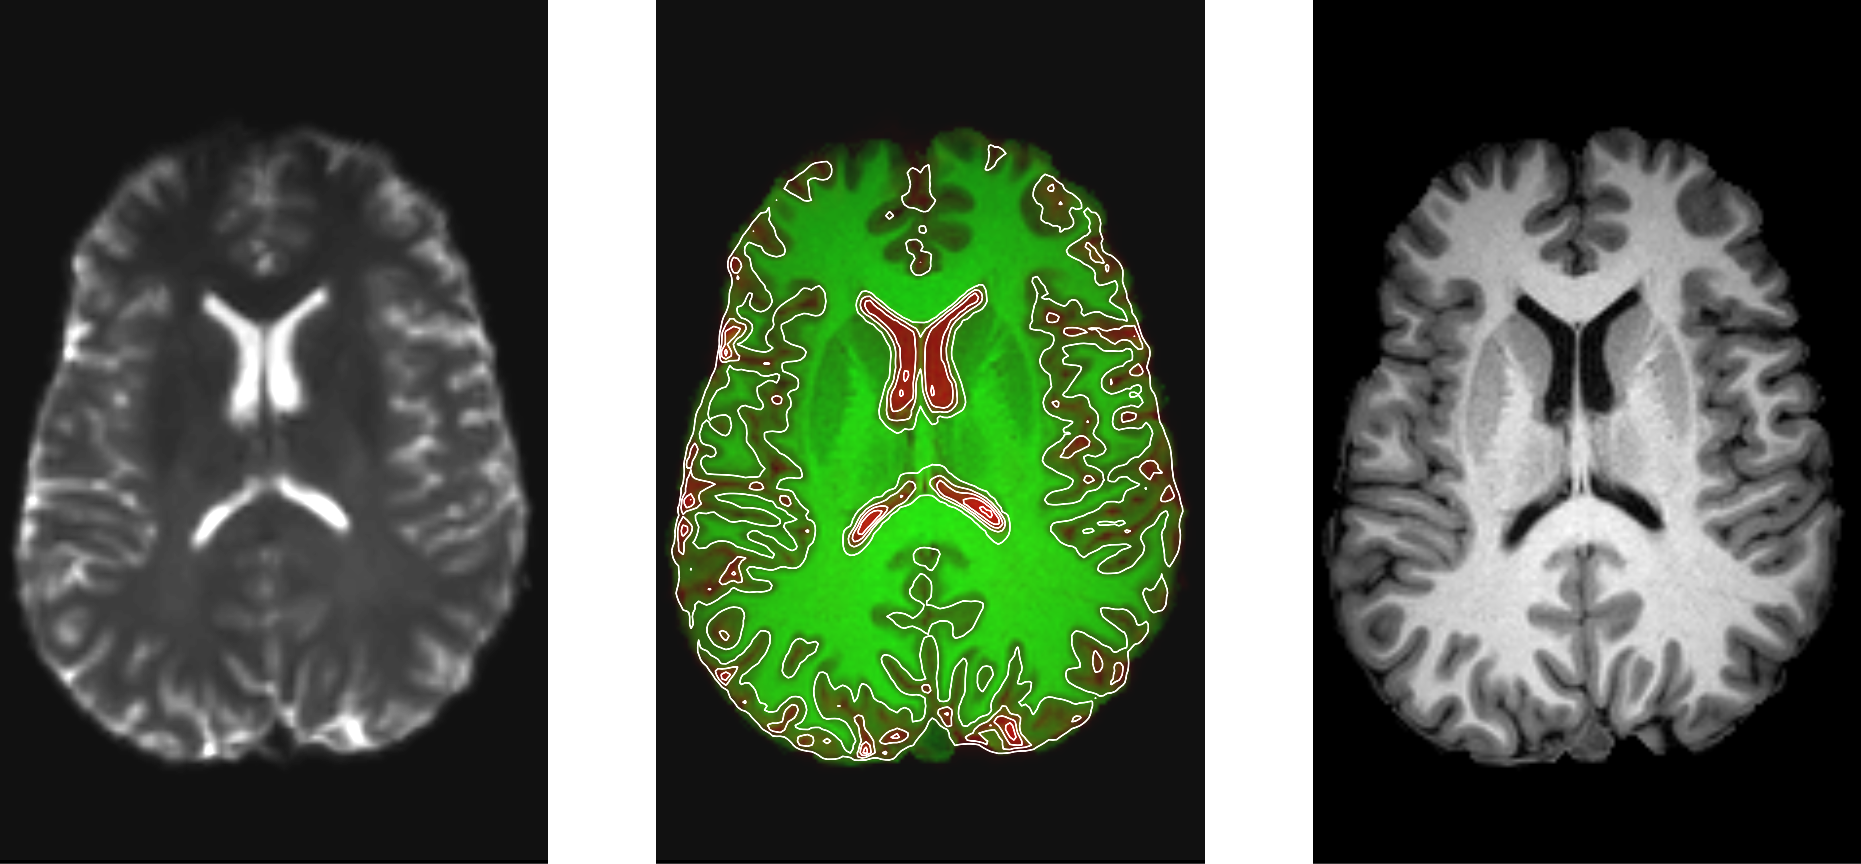
\includegraphics[width=0.55\linewidth]{./images/upt1_ecc_axial.png}}\\
    \subfloat[MI]{\label{fig:1}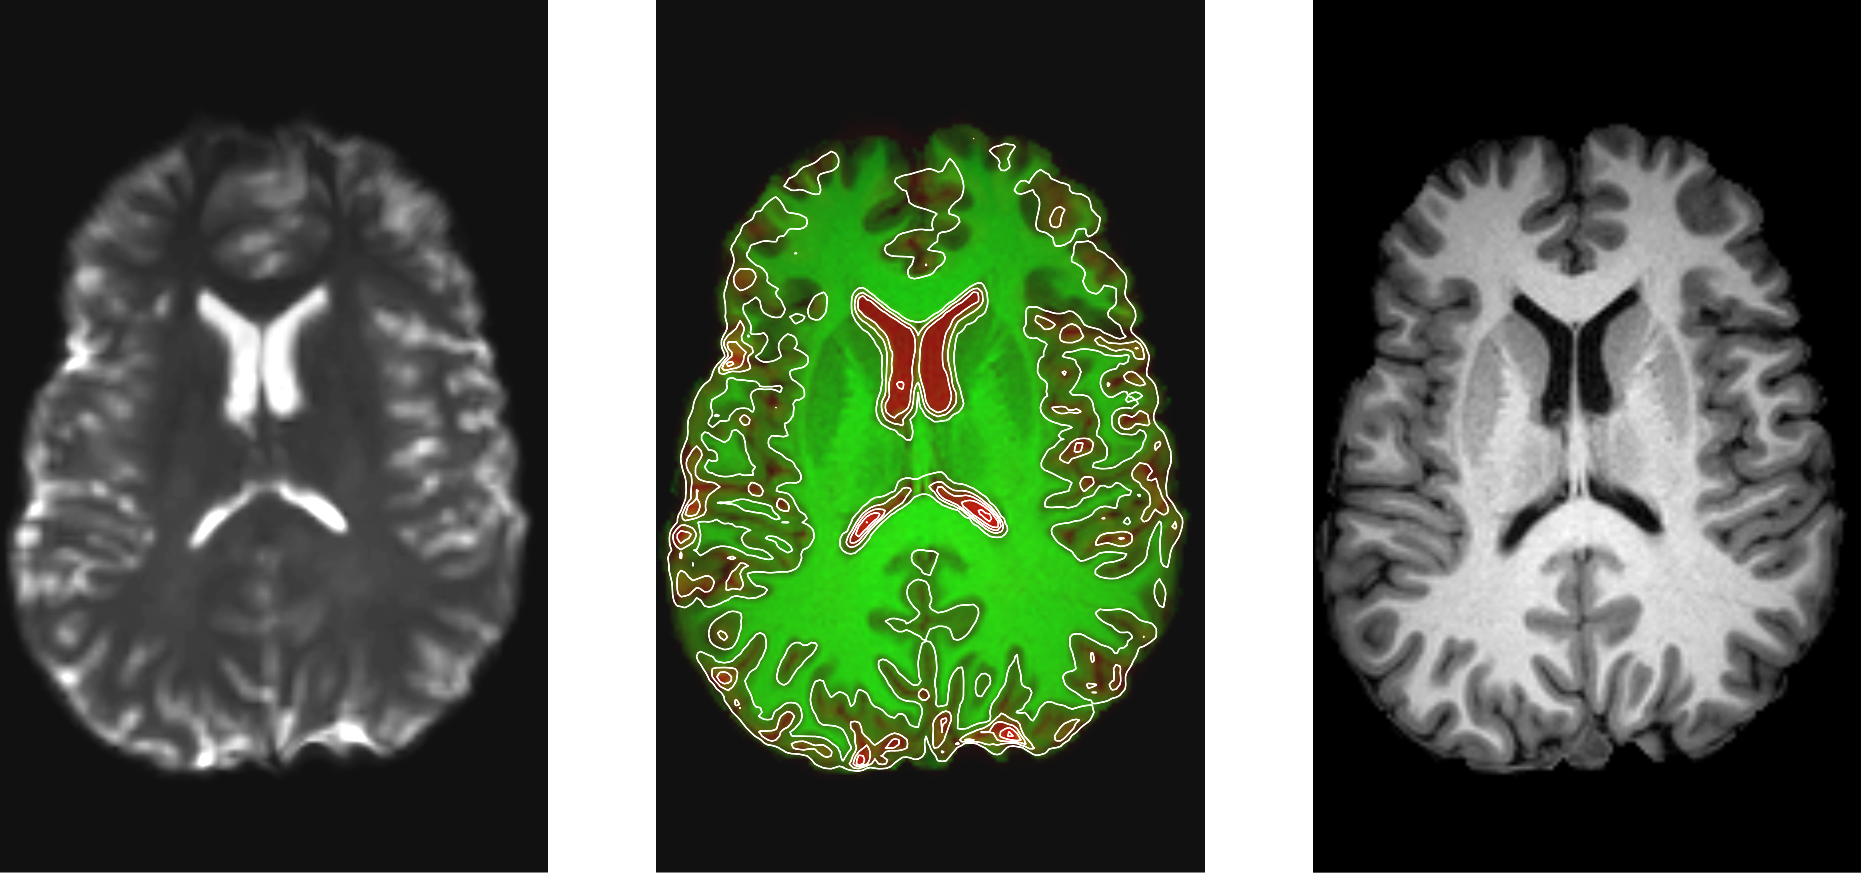
\includegraphics[width=0.55\linewidth]{./images/upt1_mi_axial.png}}\\
    \subfloat[EM]{\label{fig:1}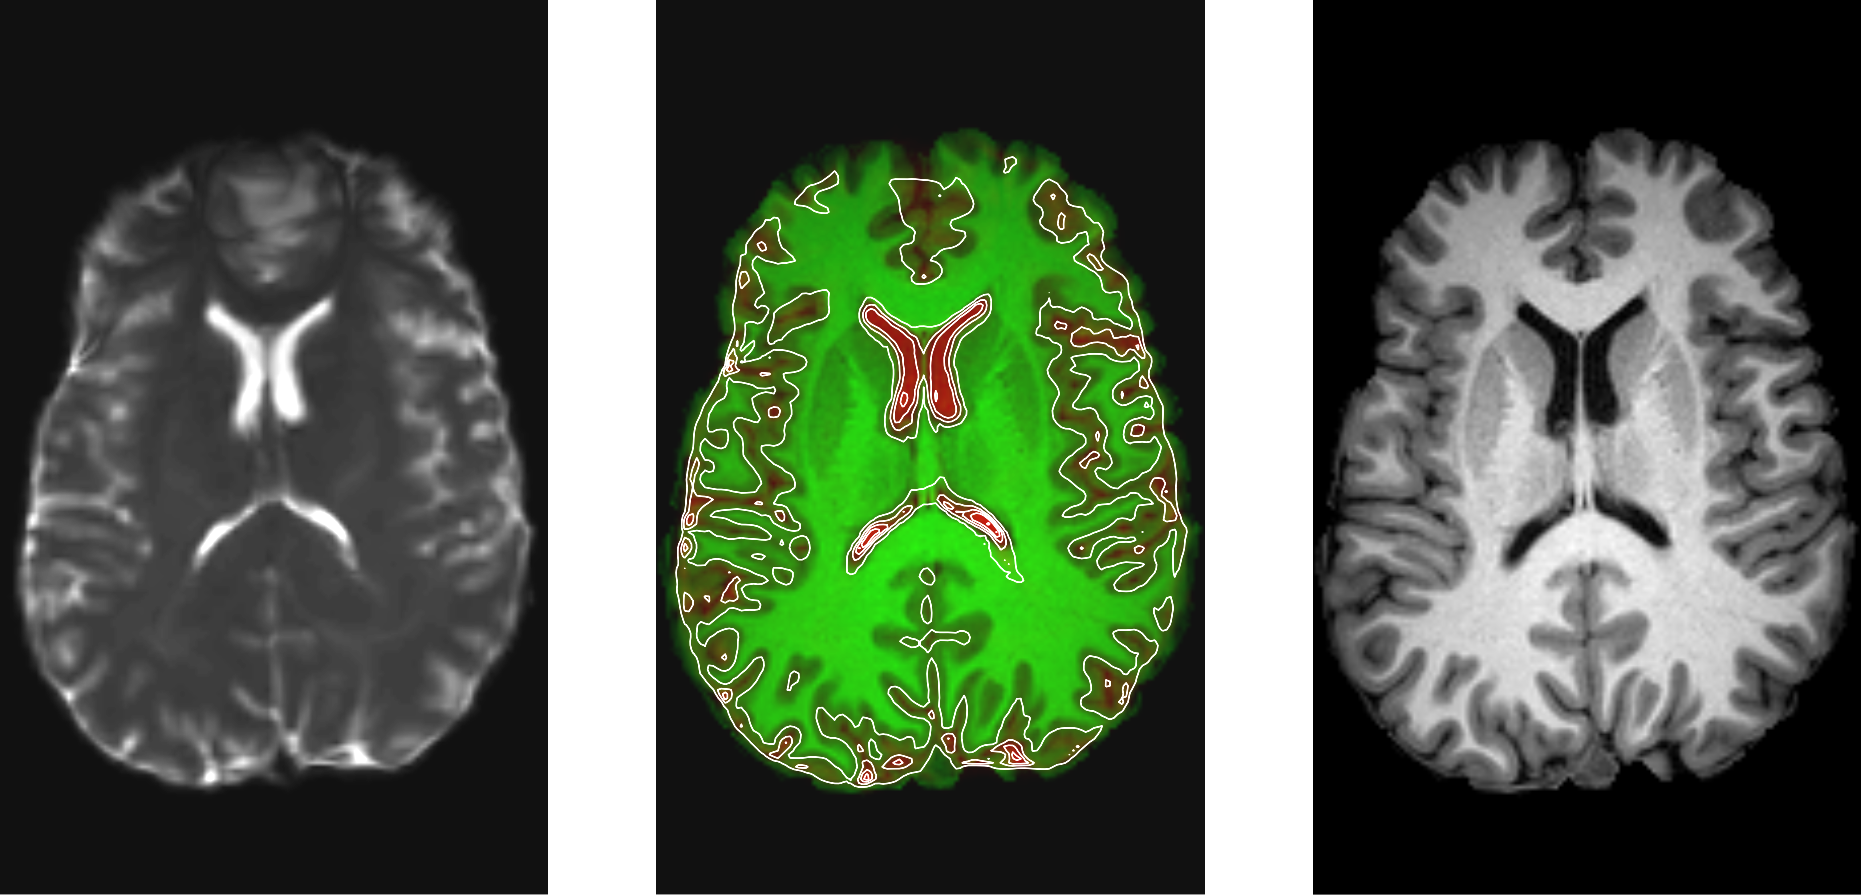
\includegraphics[width=0.55\linewidth]{./images/upt1_em_axial.png}}\\
    \subfloat[CC]{\label{fig:1}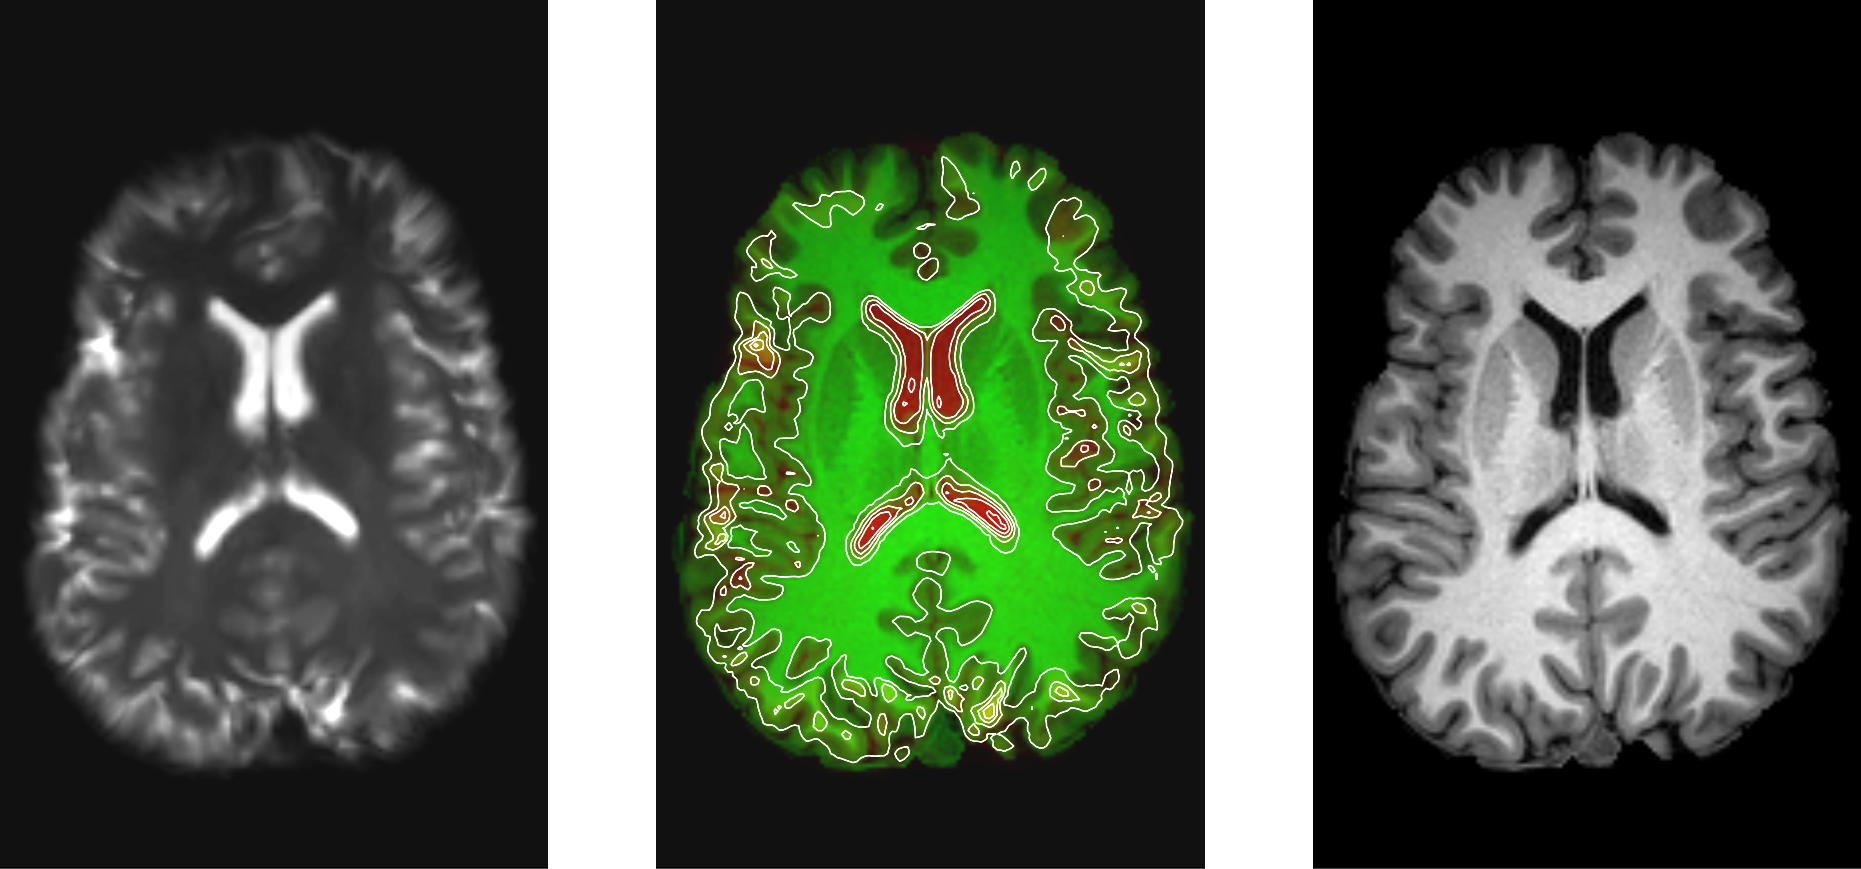
\includegraphics[width=0.55\linewidth]{./images/upt1_cc_axial.png}}\\
    \caption{Left: Warped $B_{0}$ images using SyN with each matching functional. Center: Warped $B_{0}$ (red channel) overlaid on top of the T1 (green channel) image. Level curves of the warped $B_{0}$ were overlaid on top of the T1 to visually assess local structure agreement. Right: T1 image. Visually, level curves obtained with ECC have a better correspondence with the structure of the T1.}
\label{fig:axial_examples}\figcloser
\end{figure*}

\begin{figure*}[h!]
\centering
    \subfloat[ECC]{\label{fig:1}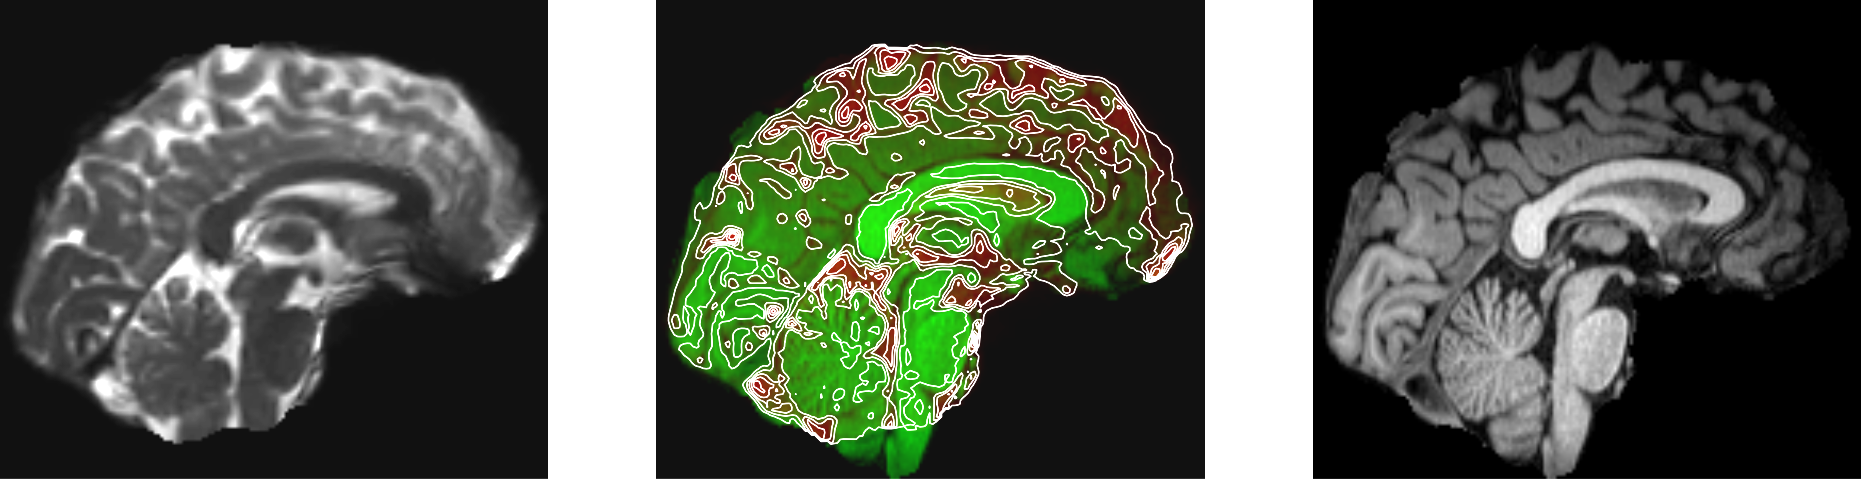
\includegraphics[width=0.8\linewidth]{./images/upt1_ecc_sagital.png}}\\
    \subfloat[MI]{\label{fig:1}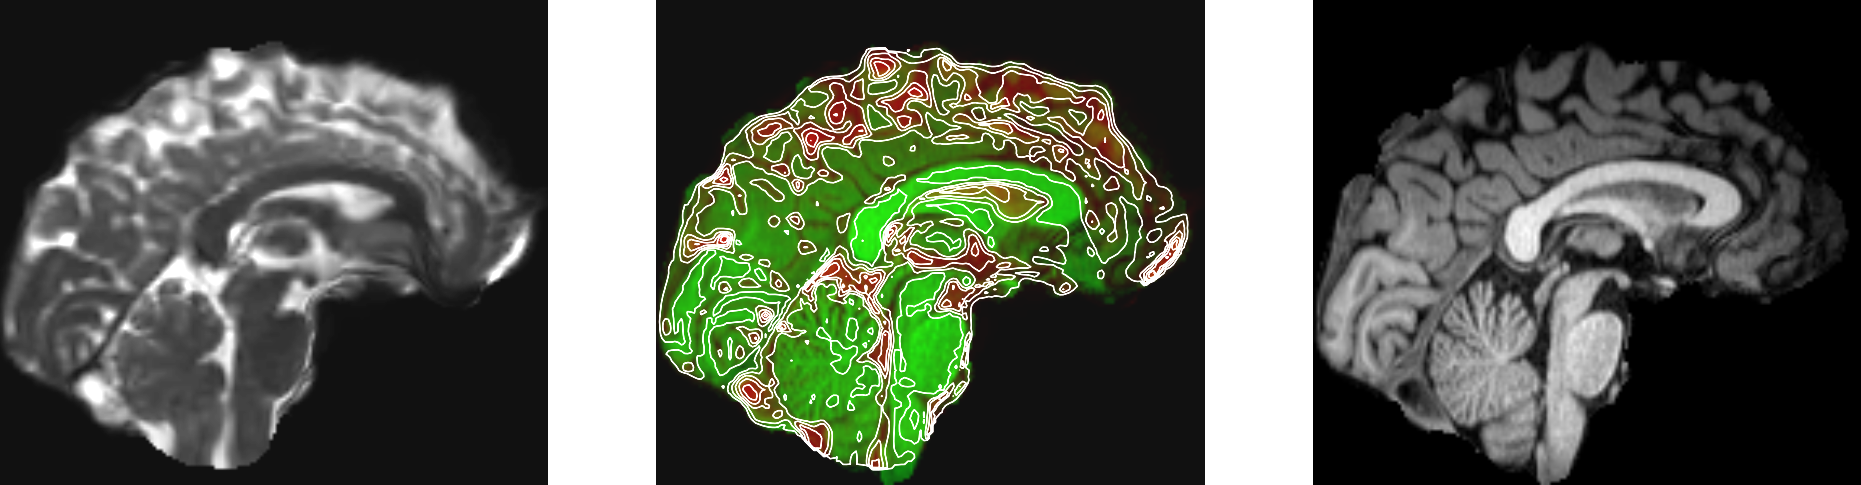
\includegraphics[width=0.8\linewidth]{./images/upt1_mi_sagital.png}}\\
    \subfloat[EM]{\label{fig:1}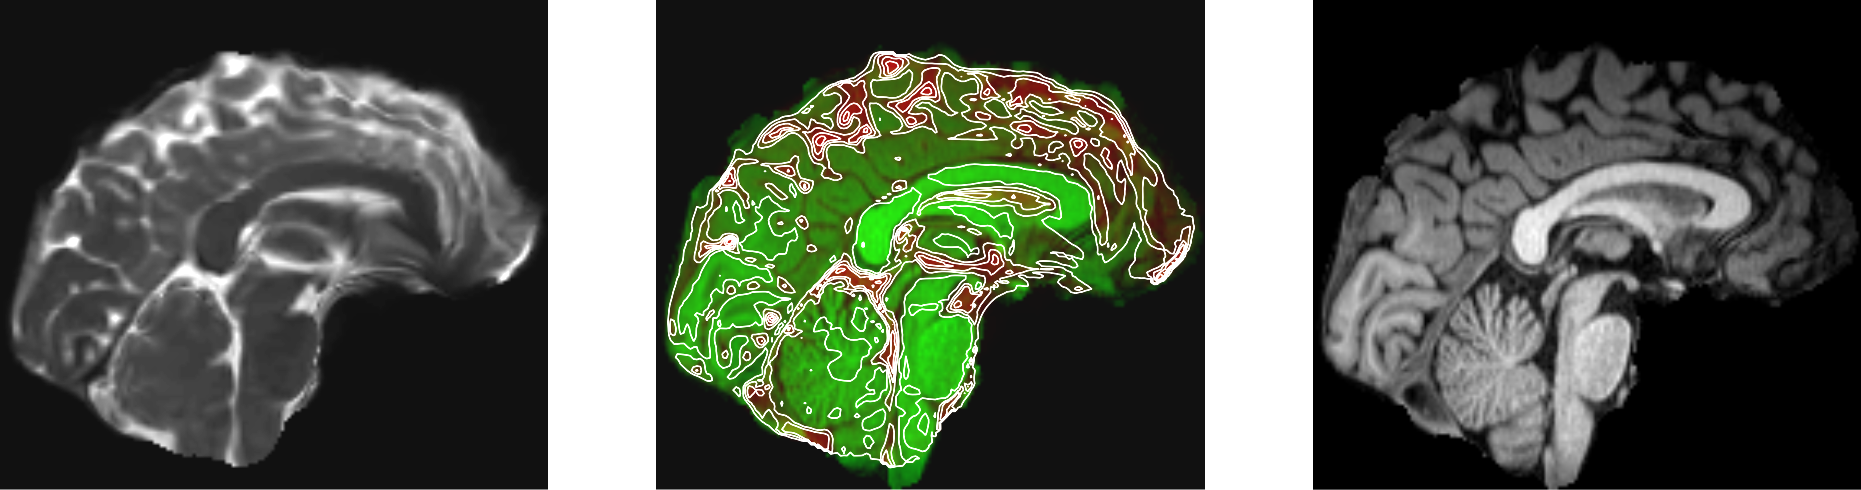
\includegraphics[width=0.8\linewidth]{./images/upt1_em_sagital.png}}\\
    \subfloat[CC]{\label{fig:1}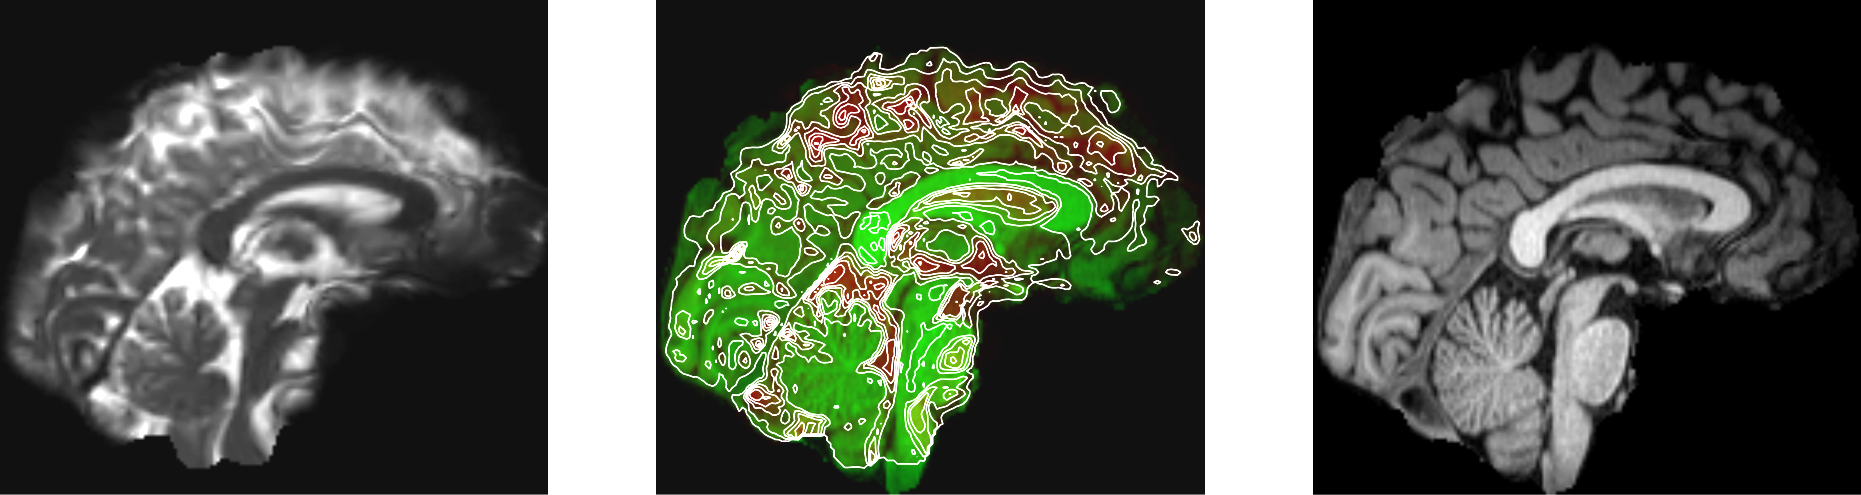
\includegraphics[width=0.8\linewidth]{./images/upt1_cc_sagital.png}}\\
    \caption{Left: Warped $B_{0}$ images using SyN with each matching functional. Center: Warped $B_{0}$ (red channel) overlaid on top of the T1 (green channel) image. Level curves of the warped $B_{0}$ were overlaid on top of the T1 to visually assess local structure agreement. Right: T1 image. Visually, level curves obtained with ECC have a better correspondence with the structure of the T1.}
\label{fig:sagital_examples}\figcloser
\end{figure*}

\begin{figure*}[h!]
\centering
    \subfloat[ECC]{\label{fig:1}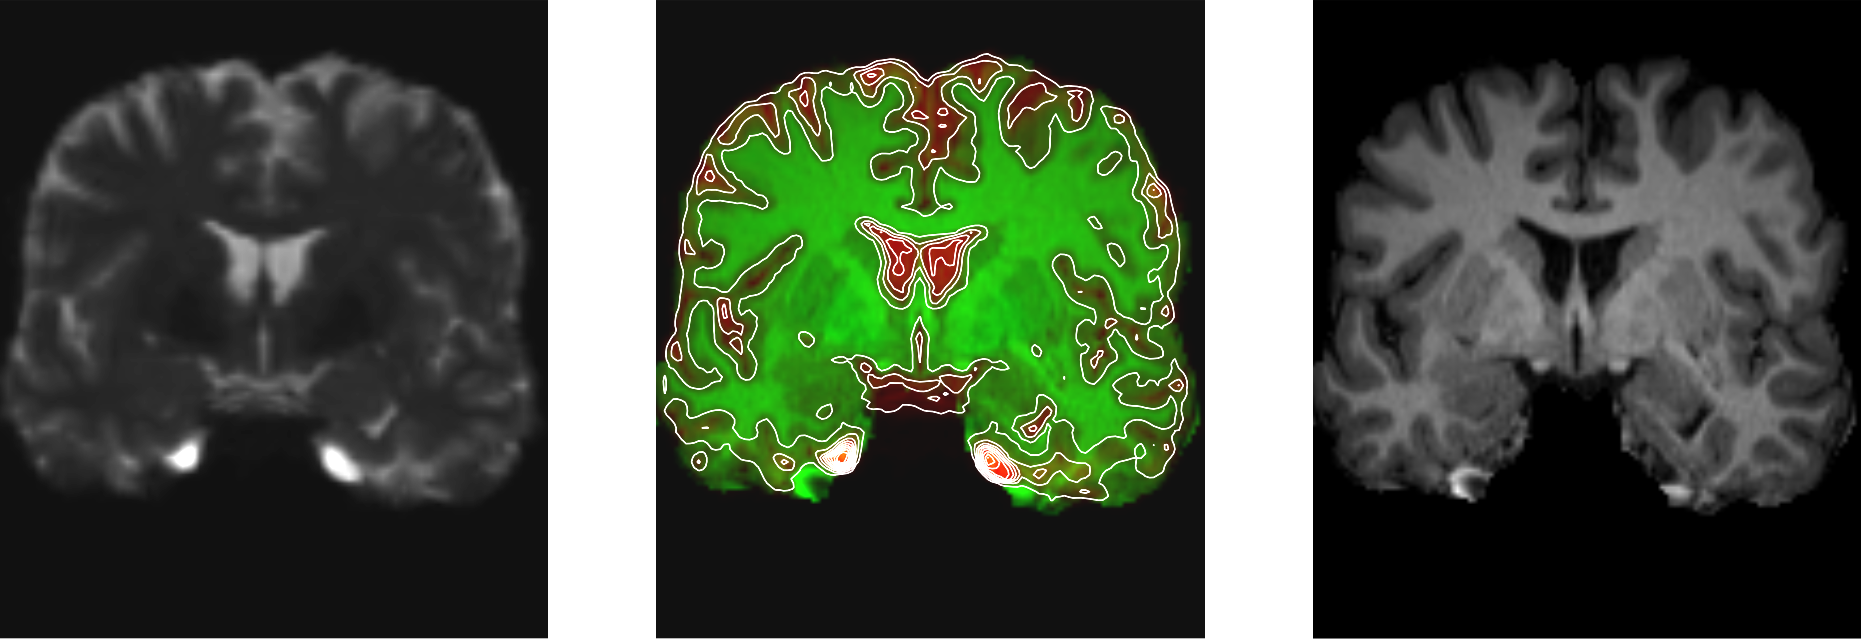
\includegraphics[width=0.8\linewidth]{./images/upt1_ecc_coronal.png}}\\
    \subfloat[MI]{\label{fig:1}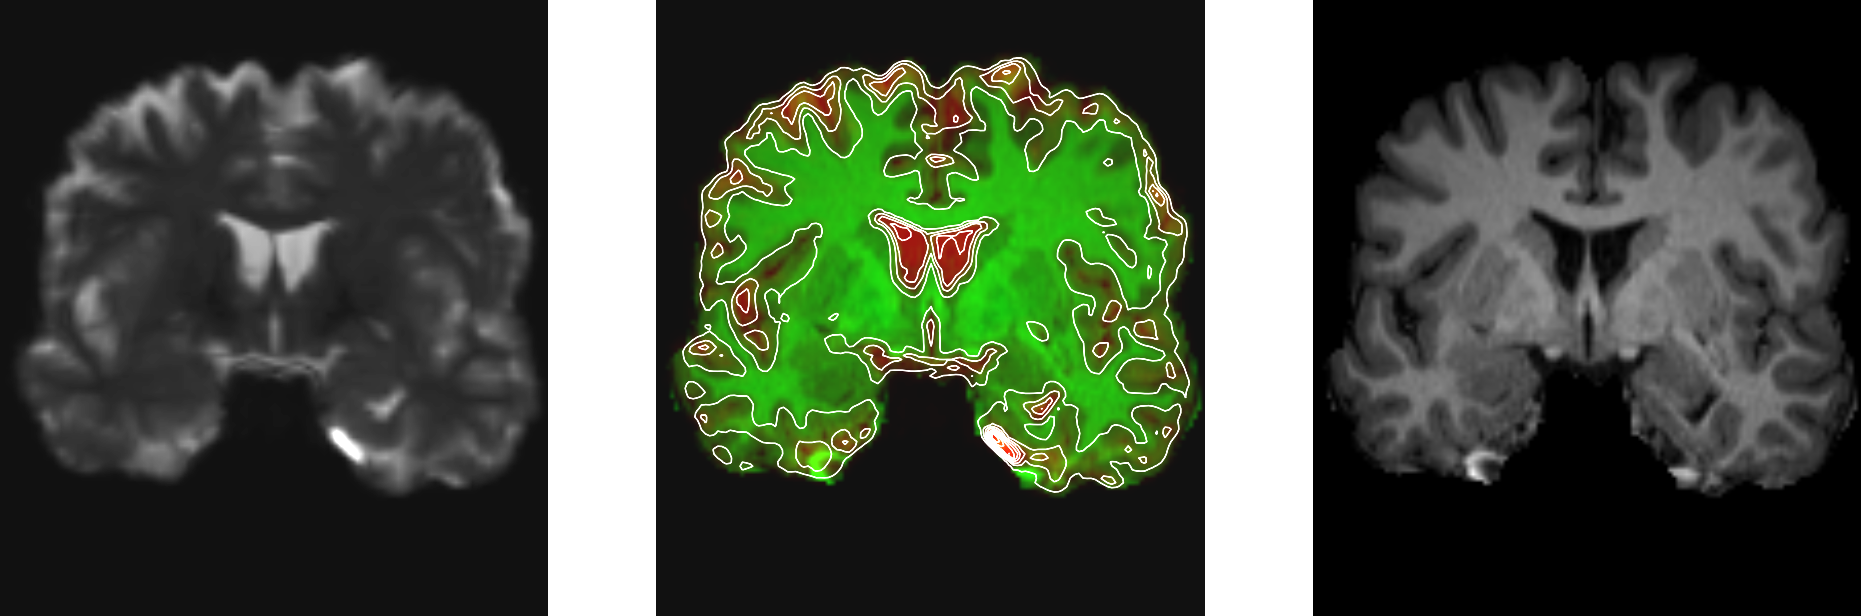
\includegraphics[width=0.8\linewidth]{./images/upt1_mi_coronal.png}}\\
    \subfloat[EM]{\label{fig:1}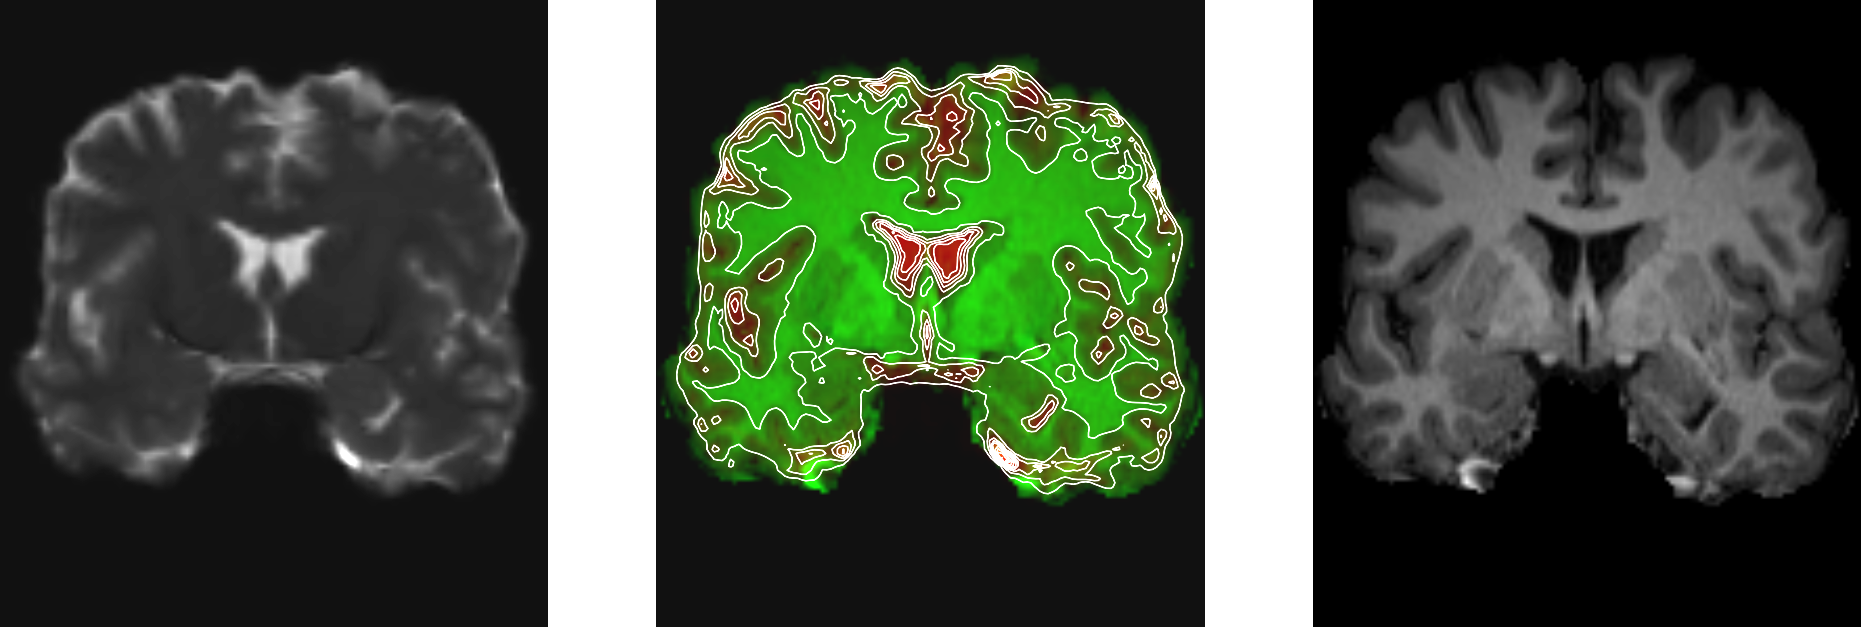
\includegraphics[width=0.8\linewidth]{./images/upt1_em_coronal.png}}\\
    \subfloat[CC]{\label{fig:1}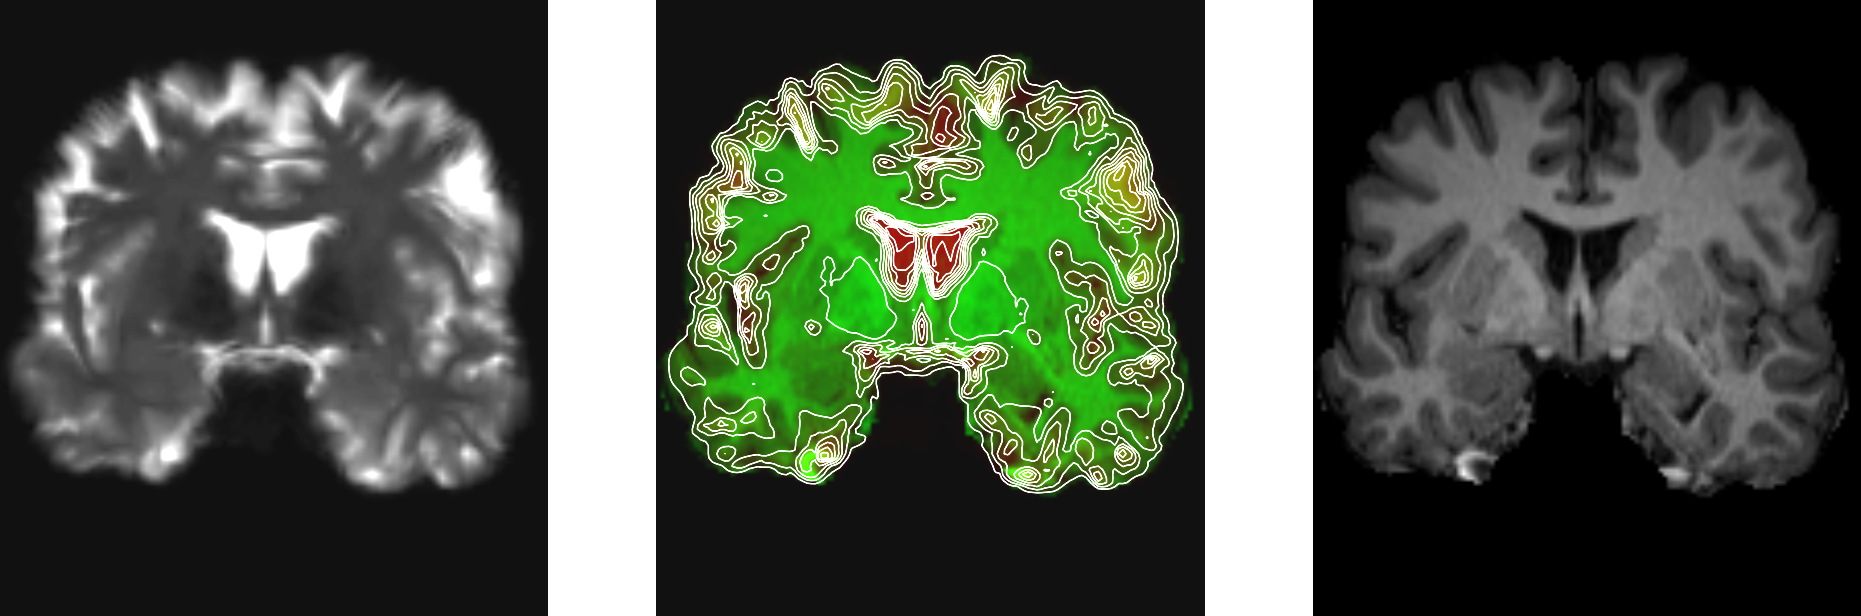
\includegraphics[width=0.8\linewidth]{./images/upt1_cc_coronal.png}}\\
    \caption{Left: Warped $B_{0}$ images using SyN with each matching functional. Center: Warped $B_{0}$ (red channel) overlaid on top of the T1 (green channel) image. Level curves of the warped $B_{0}$ were overlaid on top of the T1 to visually assess local structure agreement. Right: T1 image. Visually, level curves obtained with ECC have a better correspondence with the structure of the T1.}
\label{fig:coronal_examples}\figcloser
\end{figure*}

\section{Enlarged figures}
Figures \ref{fig:llr_test}, \ref{fig:ecc_test_good} and \ref{fig:all_pairs_boxplots} are enlarged versions of figures 2, 5, and 8, respectively, in the main document. 


\begin{figure*}[t!]
\centering
    \subfloat[]{\label{fig:T1T2_affine_fit_scatter1}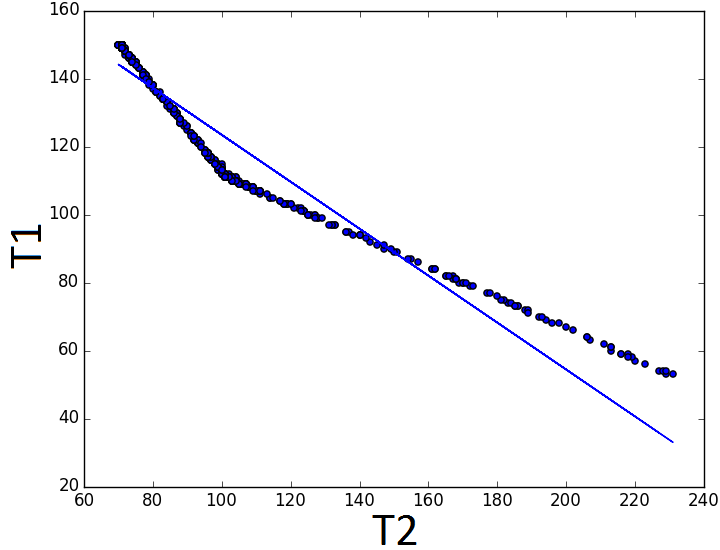
\includegraphics[width=0.2\linewidth]{./images/t1_aafo_t2_sample2.png}}
    \subfloat[]{\label{fig:T1T2_affine_fit_scatter2}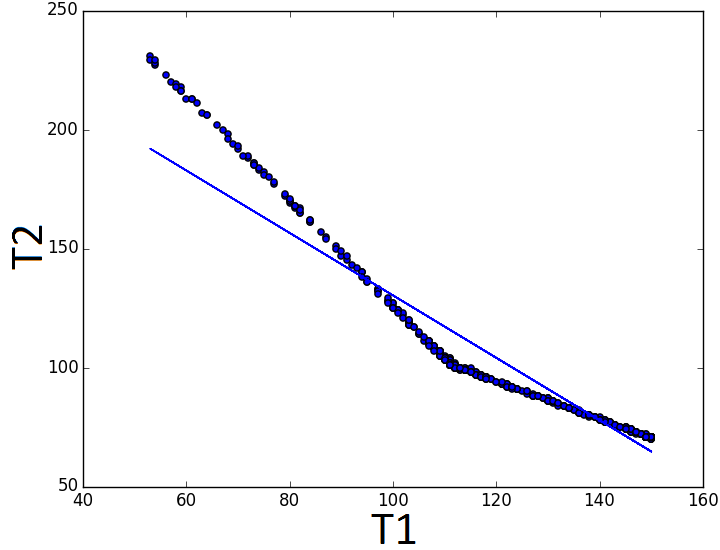
\includegraphics[width=0.2\linewidth]{./images/t2_aafo_t1_sample2.png}}
    \subfloat[]{\label{fig:T1T2_affine_fit_map}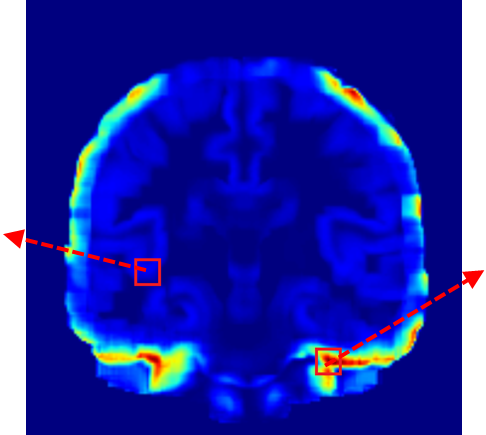
\includegraphics[width=0.2\linewidth]{./images/residuals_input_arrows.png}}
    \subfloat[]{\label{fig:T1T2_affine_fit_scatter1}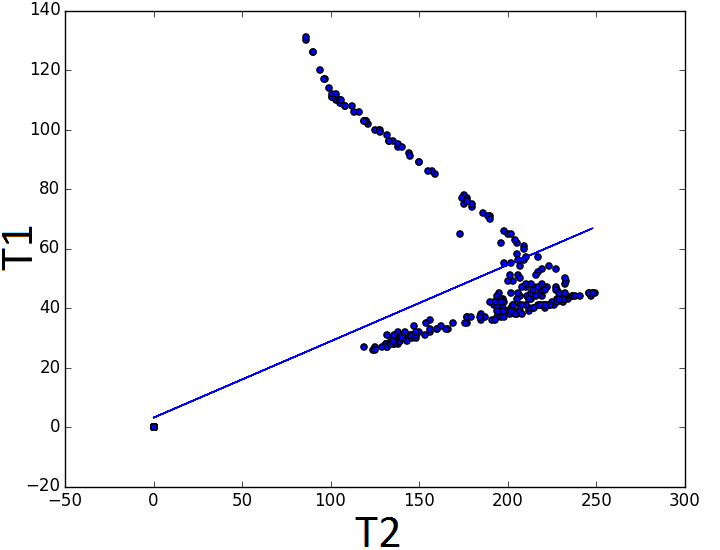
\includegraphics[width=0.2\linewidth]{./images/t1_aafo_t2_sample1.png}}
    \subfloat[]{\label{fig:T1T2_affine_fit_scatter2}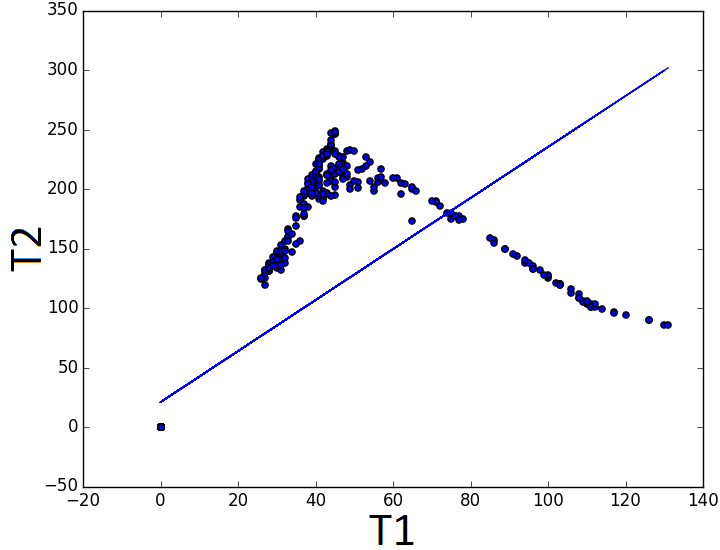
\includegraphics[width=0.2\linewidth]{./images/t2_aafo_t1_sample1.png}}\\
    \caption{{\small Local linear reconstruction between T1 and T2 images under perfect alignment (see Fig. \ref{fig:brainweb_t1_t2}). Center image (c) depicts the reconstruction error in false color. Two local windows were selected: Left (a, b): a local window with a close-to-linear relationship. Right (d, e): a local window with a far from linear relationship. The scatter plots depict the best affine fit of T1 intensities as a function of T2 (a, d), and the best fit of T2 as a function of T1 (b, e).}}
\label{fig:llr_test}\figcloser
\end{figure*}

\begin{figure*}[t]
\centering
    \subfloat[]{\label{fig:FT1T2_affine_fit_scatter1}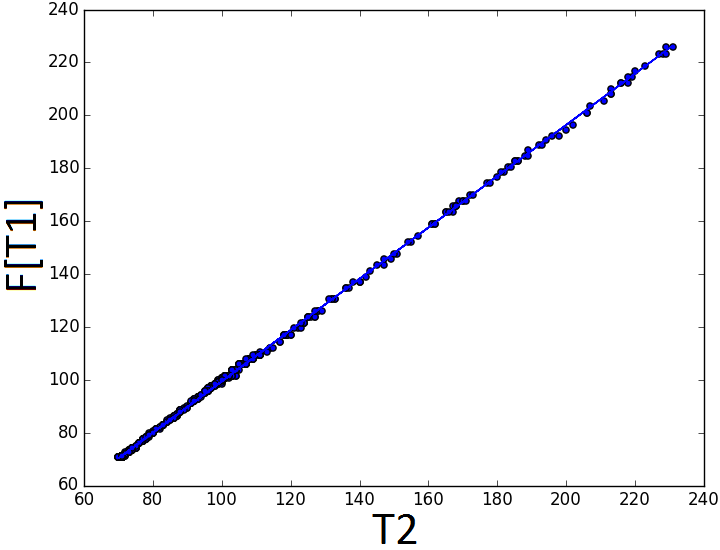
\includegraphics[width=0.2\linewidth]{./images/Ft1_aafo_t2_sample2.png}}
    \subfloat[]{\label{fig:FT1T2_affine_fit_scatter2}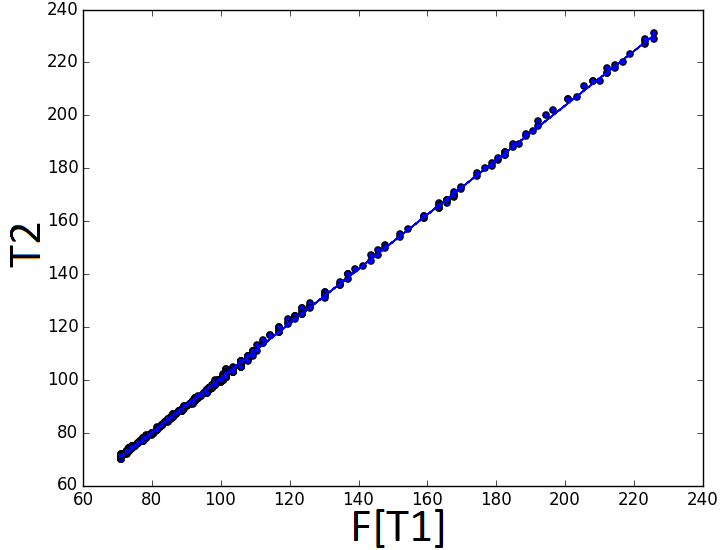
\includegraphics[width=0.2\linewidth]{./images/t2_aafo_Ft1_sample2.png}}
    \subfloat[]{\label{fig:FT1T2_affine_fit_map}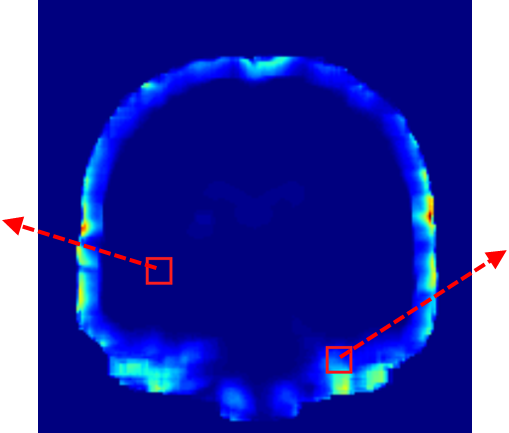
\includegraphics[width=0.2\linewidth]{./images/residuals_t2_arrows.png}}
    \subfloat[]{\label{fig:FT1T2_affine_fit_scatter1}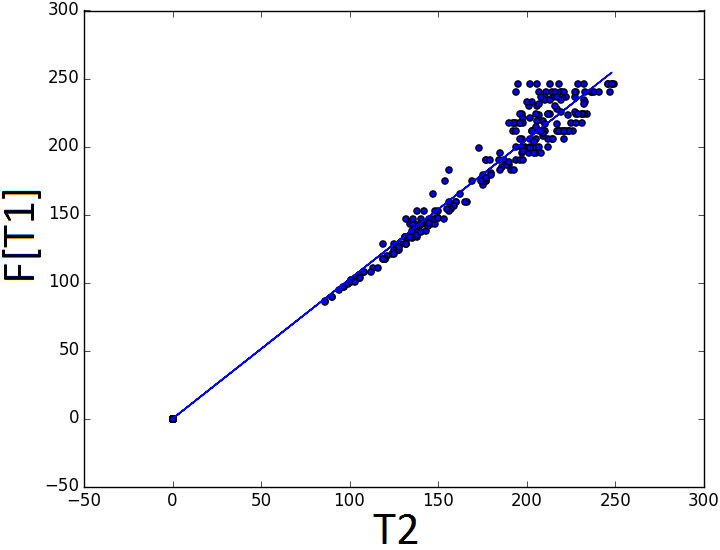
\includegraphics[width=0.2\linewidth]{./images/Ft1_aafo_t2_sample1.png}}
    \subfloat[]{\label{fig:FT1T2_affine_fit_scatter2}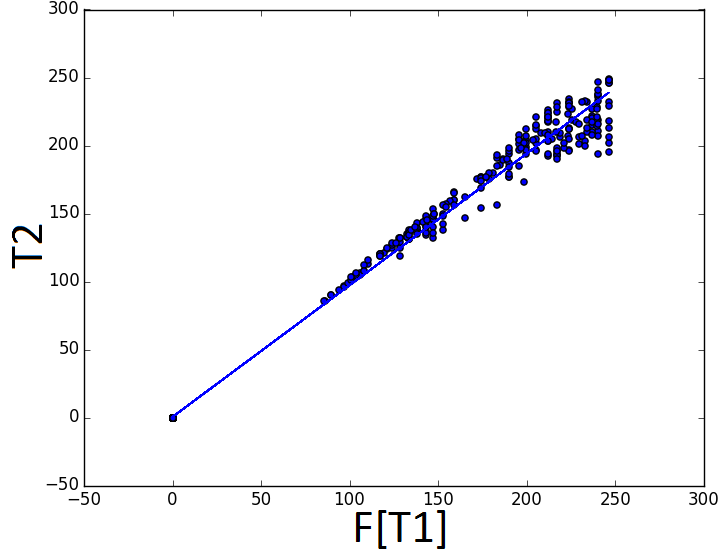
\includegraphics[width=0.2\linewidth]{./images/t2_aafo_Ft1_sample1.png}}\\
    \caption{{\small Local linear reconstruction between T2 intensities and F[T1], where F is given by $\mathbf{\bar{f}}$ (eq. \eqref{eq:average_of_isosets}). Center image (c) depicts the reconstruction error in false color. The selected windows are the same as in Fig. \ref{fig:llr_test}. The local relationship was made closer to linear by applying the global non-linear transfer F.}}
\label{fig:ecc_test_good}\figcloser
\end{figure*}

\begin{figure*}[t!]
\centering
    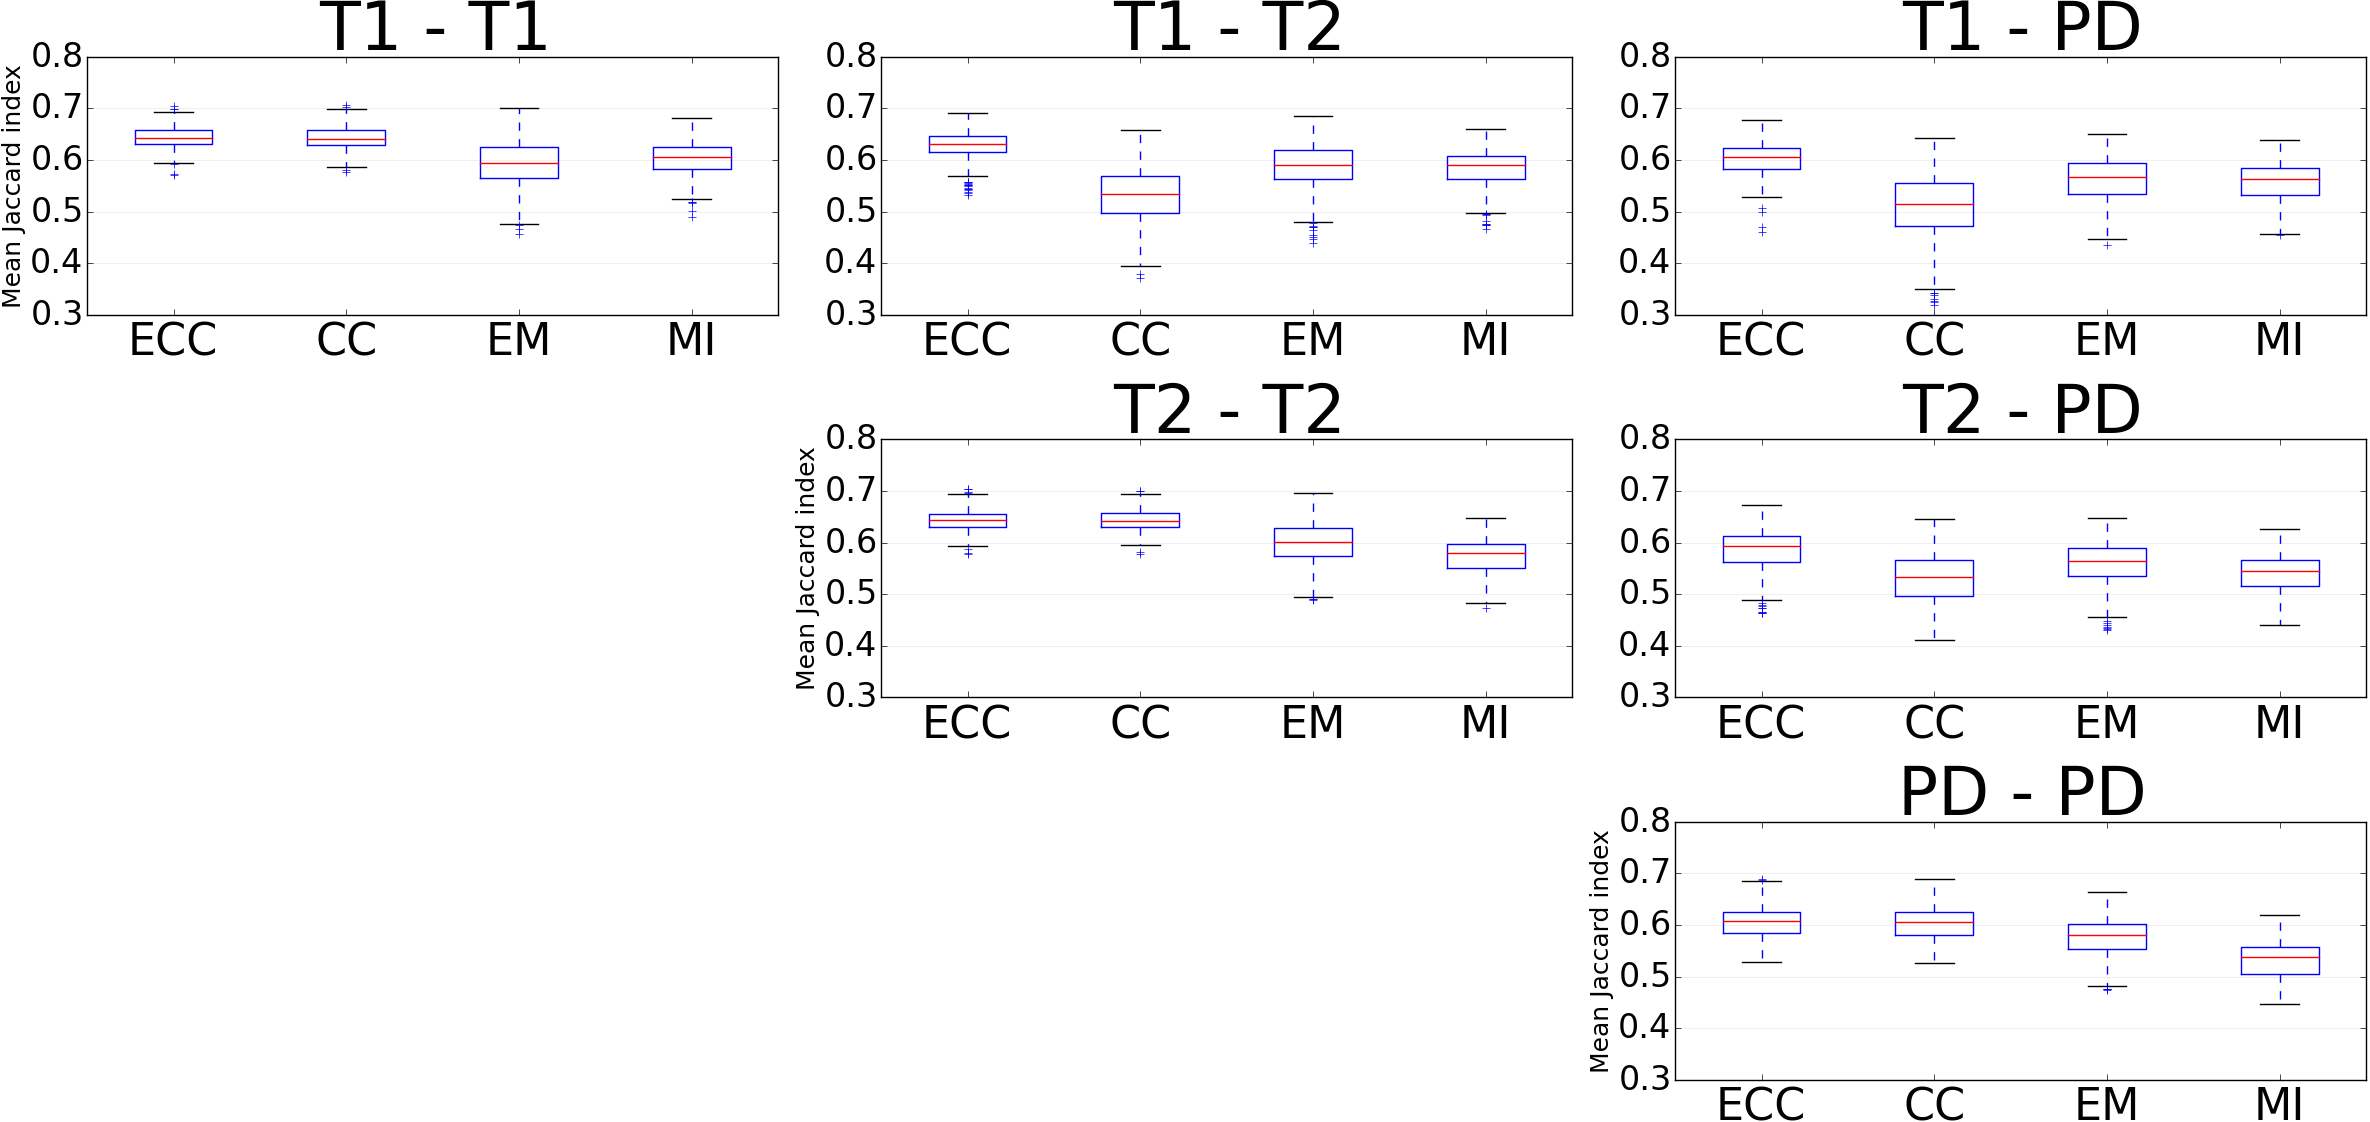
\includegraphics[width=0.75\linewidth]{./images/all_modality_pairs_boxplots.png}
    \caption{{\small Distributions of average Jaccard indices for all pairs of available modalities (T1, T2 and PD). For each pair of registrations, we compute the average Jaccard index of all anatomical regions.}}
\label{fig:all_pairs_boxplots}\figcloser
\end{figure*}

\section{Illustration of indirect validation}
In Fig. \ref{fig:indirect_validation} we illustrate the indirect validation procedure for T1-$B_0$ registration. This indirect validation allows us to measure the registration accuracy using real diffusion data (low resolution and with real noise and susceptibility-induced geometric distortions).
\begin{figure*}[t!]
\centering
    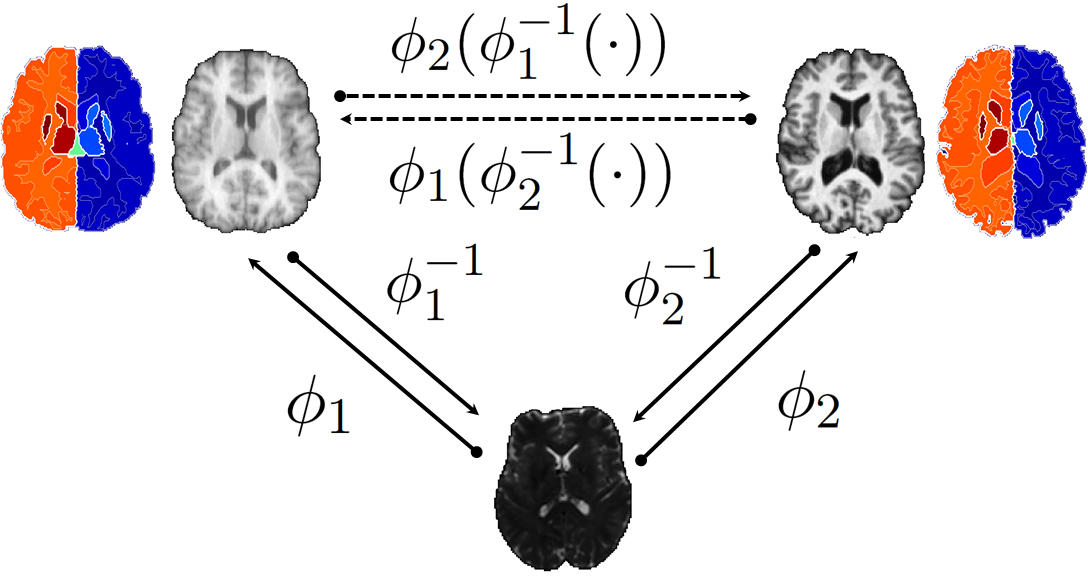
\includegraphics[width=0.75\linewidth]{./images/new_validation.png}
    \caption{{\small Indirect validation protocol for $B_{0}$-T1 registration. We first registered the $B_{0}$ (moving) image towards each T1 (fixed) annotated image, obtaining diffeomorphisms $\phi_{i}$, $i=1,2,...,18$. Then, for every pair $\phi_{i}, \phi_{j}$, we computed the composition $\phi_{i,j}:=\phi_{i}\circ \phi_{j}^{-1}$ (which now maps two annotated T1 images). The resulting overlap score indirectly measures the (combined) accuracy of both transforms.}}
\label{fig:indirect_validation}\figcloser
\end{figure*}
%\appendix{Appendices}
\section{Computation of the E-Step}\label{ap:E_step}
Here, we show the details to compute the E-step of the EM algorithm \citep{Dempster1977} to obtain a local maximum likelihood estimator for $\Phi = (\phi_{I}, \phi_{J})$.
We follow similar steps as \cite{Arce-santana2014}.\\

The E-step \citep{Dempster1977} consists in computing the conditional expectation of the log-likelihood of the (complete) data $(Y, Z, \tilde{I}, \tilde{J}, \Phi)$, according to the observation model given in eq. \eqref{eq:SyNEM_gom_update}, where $Y, Z$ are hidden random fields modeling the (unknown) transfer functions between both modalities \hbox{(eq. \eqref{eq:hidden_fields})}. A consequence of the transformations $\phi_{I}, \phi_{J}$ being diffeomorphisms (in particular, invertible) is that the domains $\Omega_{I}, \Omega_{J}$ satisfy \hbox{$\phi_{I}(\Omega_{I}) = \Omega_{R} = \phi_{J}(\Omega_{J})$} (see Fig. \ref{fig:syn_overview}). This implies that $\tilde{I}$ is independent from $\phi_{I}$, because the event $\left\lbrace I(\phi_{I}^{-1}(x)) : x\in \Omega_{R} \right\rbrace$ is equal to the event $\left\lbrace I(y) : y\in \Omega_{I} \right\rbrace$, therefore:
\begin{equation}\label{eq:image_transform_independence}
     P(\tilde{I} | \Phi) = P(I | \Phi) = P(I).
\end{equation}
It is possible to obtain a similar independence property by making a weaker (injectivity, not necessarily invertibility) assumption \citep[see][pg. 73]{Roche2000}\\

We will assume that, when the transformations $\Phi=(\phi_{I}, \phi_{J})$ are known, the random fields $(Y, \tilde{I})$ are independent from $(Z, \tilde{J})$. In other words, once we know $\Phi$, any knowledge of $(Z, \tilde{J})$ no longer provide any additional information regarding the distribution of $(Y, \tilde{I})$, and viceversa. More precisely:
\begin{equation}\label{eq:conditional_independence_assumption}
    P(\tilde{I}, \tilde{J}, Y, Z | \Phi) = P(\tilde{I}, Y | \Phi)P(\tilde{J}, Z| \Phi).
\end{equation}
From eq. \eqref{eq:image_transform_independence}, it follows that
\begin{equation}\label{eq:joint_to_conditional}
    P(\tilde{I}, Y | \Phi) = P(Y | \tilde{I}, \Phi)P(\tilde{I} | \Phi) = P(Y | I, \Phi)P(I),
\end{equation}
similarly, $P(\tilde{J}, Z| \Phi) = P(Z| J, \Phi)P(J)$. From eqs. \eqref{eq:conditional_independence_assumption} and \eqref{eq:joint_to_conditional} we obtain
\begin{equation}\label{eq:simplified_joint_prob}
    P(\tilde{I}, \tilde{J}, Y, Z, \Phi) = P(Y | I, \Phi)P(Z| J, \Phi)P(\Phi)P(I)P(J).
\end{equation}

The conditional expectation of the log-likelihood (of the complete data) evaluated on an initial parameter $\Phi^{(0)}$ can be simplified using eq. \eqref{eq:simplified_joint_prob} as follows:
\begin{displaymath}
    Q(\Phi; \Phi^{(0)}) := \mathbbm{E}\left[\left. \log \left(P(\tilde{I}, \tilde{J}, Y, Z, \Phi)\right) \right | I, J, \Phi^{(0)}\right] =
\end{displaymath}
\begin{displaymath}
    \mathbbm{E}\left[\left. \log \left(P(Y |I, \Phi)P(Z|J, \Phi)P(\Phi)P(I)P{J}\right) \right | I, J, \Phi^{(0)}\right] =
\end{displaymath}
\begin{equation}\label{eq:separated_expectations}
    -R(\Phi) + C + \mathbbm{E}\left[ \log \left(P(Y|I, \Phi)\right) | I, J, \Phi^{(0)}\right] + \mathbbm{E}\left[ \log \left(P(Z|J, \Phi)\right) | I, J, \Phi^{(0)}\right]
\end{equation}
where $R(\Phi) = -\log P(\Phi)$ is known as the ``regularization term'', and \hbox{$C=\log \left(P(I)P(J)\right)$} is a constant that does not depend on $\Phi$. For simplicity, we will elaborate on the first expectation only, the second can be computed analogously.\\

By definition, the random field $\eta_{J}$ is a set of independent, zero-mean, Normally-distributed random variables. More precisely, if $f_{x}:\mathbf{R}\rightarrow \mathbf{R}^{+}$ is the probability density
function of $\eta_{J}(x)$ then:
\begin{equation}\label{eq:gaussian}
    f_{x}(u) = \frac{1}{\sigma_{Y}(x)\sqrt{2 \pi}}\exp\left(-\frac{u^{2}}{2\sigma^{2}_{Y}(x)}\right)
\end{equation}
and, from our observation model (eq. \eqref{eq:SyNEM_gom_update}), it follows that:
\begin{equation}
    P(Y(x)| I, \Phi) = P(\eta_{J}(x) = Y(x)-\tilde{I}(x)) = f_{x}(Y(x)-\tilde{I}(x)).
\end{equation}
Therefore, the joint conditional probability of $Y$ given $I, \Phi$ is the product of the above marginals:
\begin{equation}\label{eq:Y_field_cond_indep}
    P(Y|I, \Phi) = \prod_{x\in{\Omega_{R}}} f_{x}(Y(x) - \tilde{I}(x)),
\end{equation}
and the first conditional expectation of eq. \eqref{eq:separated_expectations} can be writen as:
\begin{equation}
    Q_{I}(\phi_{I} ; \Phi^{(0)}) := \int_{\mathcal{Y}}\left[\sum_{x\in\Omega_{R}} \log f_{x}\left(y(x) - \tilde{I}(x)\right) \right] dP(y | I, J, \Phi^{(0)}),
\end{equation}
where $\mathcal{Y}$ is the set of all possible configurations of the vector field $Y$. By assuming a finite grid $\Omega_{R}$, we may interchange the order of summation and integration, which yields:
\begin{equation}\label{eq:data_term}
    Q_{I}(\phi_{I} ; \Phi^{(0)}) = \sum_{x\in\Omega_{R}} \int_{\mathcal{Y}} \log f_{x}\left(y(x) - \tilde{I}(x)\right)  dP(y | I, J, \Phi^{(0)}).
\end{equation}

Since all the variables $Y(x), x\in\Omega_{R}$ are conditionally independent given $I, \Phi^{(0)}$ (eq. \eqref{eq:Y_field_cond_indep}), we have $P(y | I, J, \Phi^{(0)}) = P(y(x)| I, J, \Phi^{(0)})P(y^{C}(x) | I, J, \Phi^{(0)})$, where the complement $Y^{C}(x)$
denotes the subset of random variables other than $Y(x)$, and $y^{C}(x)$ is a configuration of $Y^{C}(x)$. Therefore, the right-hand side of eq.\eqref{eq:data_term} can be written as

\begin{equation}\label{eq:split_integral}
    \sum_{x\in\Omega_{R}} \int_{\mathcal{Y}^{C}(x)} \left[\int_{\mathbf{R}} \log f_{x}\left(\ell - \tilde{I}(x)\right) P(Y(x) = \ell | I, J, \Phi^{(0)})d\ell\right]  dP(y^{C}(x) | I, J, \Phi^{(0)})
\end{equation}
where $\mathcal{Y}^{C}(x)$ is the set of all possible configurations of $Y^{C}(x)$.\\

Since \hbox{$\int_{\mathcal{Y}^{C}(x)}dP(y^{C}(x) | I, J, \Phi^{(0)}) = 1$}, and the inner integral
is an expected value w.r.t. the conditional distribution:
\begin{equation}
     Q_{I}(\phi_{I} ; \Phi^{(0)}) = \sum_{x\in\Omega_{R}} \mathbbm{E} \left[\left.\log f_{x}\left(Y(x) - \tilde{I}(x)\right) \right| I, J, \Phi^{(0)}\right].
\end{equation}
By expanding the density function (according to eq. \eqref{eq:gaussian}) and denoting by $\overline{Y}(x), \widehat{\sigma^{2}_{Y}(x)}$ the conditional mean and variance of $Y(x)$
given the data and fixed parameters $\Phi^{(0)}$, we have
\begin{equation}
    \mathbbm{E} \left[\left.\log \frac{1}{\sigma_{Y}(x)\sqrt{2\pi}} - \frac{(Y(x) - I(\phi^{-1}_{I}(x)))^{2}}{2\sigma^{2}_{Y}(x)}\right|I, J, \Phi^{(0)} \right] =
\end{equation}
\begin{equation}
    = \log \frac{1}{\sigma_{Y}(x)\sqrt{2\pi}} - \mathbbm{E} \left[\left. \frac{(Y(x) - \overline{Y}(x) + \overline{Y}(x) - I(\phi^{-1}_{I}(x)))^{2}}{2\sigma^{2}_{Y}(x)}\right|I, J, \Phi^{(0)} \right]=
\end{equation}
%\begin{equation}
%    = \log \frac{1}{\sigma_{Y}(x)\sqrt{2\pi}} - \mathbbm{E} \left[\left. \frac{(Y(x) - \overline{Y}(x))^{2}+ (\overline{Y}(x) - I(\phi^{-1}_{I}(x)))^{2} - 2(Y(x) - \overline{Y}(x)) (\overline{Y}(x) - I(\phi^{-1}_{I}(x)))}{2\sigma^{2}_{Y}(x)}\right|I, J, \Phi^{(0)} \right]=
%\end{equation}
\begin{equation}
    = \log \frac{1}{\sigma_{Y}(x)\sqrt{2\pi}} - \frac{\widehat{\sigma^{2}_{Y}(x)} + (\overline{Y}(x) - I(\phi^{-1}_{I}(x)))^{2}}{2\sigma^{2}_{Y}(x)}.
\end{equation}
Finally, by approximating the (unknown) parameters $\sigma_{Y}(x)$ by $\widehat{\sigma_{Y}(x)}$ we obtain:
\begin{equation}
    Q_{I}(\phi_{I} ; \Phi^{(0)}) = C_{I} - \sum_{x\in\Omega_{x}}\frac{(\overline{Y}(x) - I(\phi^{-1}_{I}(x)))^{2}}{2\widehat{\sigma^{2}_{Y}(x)}},
\end{equation}
where $C_{I} = -\frac{1}{2} - \log\left(\widehat{\sigma^{2}_{Y}(x)}\sqrt{2\pi}\right)$ is a constant that depends on the (known) initial transformations $\Phi^{(0)}$, but not on the (unknown) transformation $\phi_{I}$ we wish to optimize. Image $\overline{Y}$ may be regarded as an approximation of image $\tilde{I}$, since it can be efficiently computed by assigning to $\overline{Y}(x)$ the average intensity of the iso-set $\left\lbrace \tilde{I}(y) : \tilde{J}(y) = \tilde{J}(x)\right\rbrace$ \citep{Roche1998}. The conditional variance $\widehat{\sigma^{2}_{Y}}(x)$ measures the uncertainty at each point $x\in \Omega_{R}$.\\

Similarly, if $\overline{Z}(x), \widehat{\sigma^{2}_{Z}(x)}$ are the conditional mean and variance of $Z(x)$ given the data
and fixed parameters $\Phi^{(0)}$, the second conditional expectation of eq. \eqref{eq:separated_expectations} can be writen as

\begin{equation}
    Q_{J}(\phi_{J}; \Phi^{(0)}) = C_{J} - \sum_{x\in\Omega_{x}}\frac{(\overline{Z}(x) - J(\phi^{-1}_{J}(x)))^{2}}{2\widehat{\sigma^{2}_{Z}(x)}}.
\end{equation}
If we choose a regularization function of the form $R(\Phi) = \lambda R_{I}(\phi_{I}) + \lambda R_{J}(\phi_{J})$ the final function to be \textbf{maximized} in the M step is given by

\begin{equation}
    Q(\Phi; \Phi^{(0)}) = \left[Q_{I}(\phi_{I}; \Phi^{(0)}) - \lambda R_{I}(\phi_{I})\right] + \left[Q_{J}(\phi_{J}; \Phi^{(0)}) - \lambda R_{J}(\phi_{J})\right],
\end{equation}
which is the sum of two independent cost functions for $\phi_{I}$ and $\phi_{J}$.

\section{Gradient of the CC metric}\label{ap:CC_gradient}
We are interested in computing the gradient of
\begin{equation}
    CC(\bar{I}, \bar{J}, x) = \frac{<\bar{I}, \bar{J}>^{2}}{<\bar{I}><\bar{J}>}
\end{equation}
where the inner product is taken over an $n^{D}$ window \citep[see][eq. 4]{Avants2008}. Since the windows are considered discrete, a more precise notation
for this expression is:
\begin{equation}\label{eq:CC_definition}
    CC(y;\phi_{I}, \phi_{J}) = \frac{\left[\sum_{z\in W_{y}} \left(\tilde{I}(z) - \mu_{y}\right)\left(\tilde{J}(z) - \nu_{y}\right)\right]^{2}}
    {\left[\sum_{z \in W_{y}}\left(\tilde{I}(z) - \mu_{y}\right)^{2}\right] \left[\sum_{z \in W_{y}}\left(\tilde{J}(z) - \nu_{y}\right)^{2}\right]} = \frac{A_{y}^{2}}{B_{y}C_{y}}
\end{equation}
where $\tilde{I}(z) = I(\phi_{I}^{-1}(z))$, $\tilde{J}(z) = J(\phi_{J}^{-1}(z))$ and the full energy is given by
\begin{equation}
    CC(\phi_{I}, \phi_{J}) = \sum_{y\in\Omega} CC(y; \phi_{I}, \phi_{J})
\end{equation}
where $W_{y}$ is the window of side $n$ centered at voxel $y$, $|W_{y}|$ is the number of voxels in window $W_{y}$ and:
\begin{equation}
    \begin{array}{lll}
        \mu_{y} &=& \frac{1}{|W_{y}|}\sum_{z \in W_{y}}\tilde{I}(z)\\[+2mm]
        \nu_{y} &=& \frac{1}{|W_{y}|}\sum_{z \in W_{y}}\tilde{J}(z)\\
    \end{array}.
\end{equation}

We wish to compute the gradient of $CC(\phi_{I}, \phi_{J})$ with respect to $\phi^{-1}_{J}(x)$, $x\in\Omega$. The set of window terms $CC(y;\phi_{I}, \phi_{J})$
that depend on $\phi^{-1}_{J}(x)$ is precisely the set of all windows $W_{y}$ such that $y \in W_{x}$. Therefore:
\begin{equation}
    \frac{\partial CC (\phi_{I}, \phi_{J})}{\partial \phi^{-1}_{J}(x)} = \sum_{y \in W_{x}} \frac{\partial CC (y; \phi_{I}, \phi_{J})}{\partial \phi^{-1}_{J}(x)}
\end{equation}
and
\begin{equation}
    \frac{\partial CC (y; \phi_{I}, \phi_{J})}{\partial \phi^{-1}_{J}(x)} =
        \frac{\left(2A_{y} B_{y}C_{y}\right)\frac{\partial A_{y}}{\partial \phi^{-1}_{J}(x)} - \left(A_{y}^{2}B_{y}\right)\frac{\partial C_{y}}{\partial \phi^{-1}_{J}(x)}}
             {B_{y}^{2} C_{y}^{2}}
\end{equation}
where
\begin{equation}
    \begin{array}{lll}
        \frac{\partial A_{y}}{\partial \phi^{-1}_{J}(x)} &=& (\tilde{I}(x) - \mu_{y})\nabla \tilde{J}(x)\\[+3mm]
        \frac{\partial C_{y}}{\partial \phi^{-1}_{J}(x)} &=& 2(\tilde{J}(x) - \nu_{y})\nabla \tilde{J}(x)
    \end{array}.
\end{equation}
After simplifying, we get
\begin{equation}\label{eq:CC_gradient}
    \frac{\partial CC (\phi_{I}, \phi_{J})}{\partial \phi^{-1}_{J}(x)} = \sum_{y \in W_{x}}
         \frac{2A_{y}}
              {B_{y}C_{y}}\left[ (\tilde{I}(x) - \mu_{y}) - \frac{A_{y}}{C_{y}}\left(\tilde{J}(x) - \nu_{y}\right)\right]\nabla \tilde{J}(x).
\end{equation}
If we define the scalar functions
\begin{equation}
    \begin{array}{lll}
        S_{a}(x) &=& \sum_{y \in W_{x}} \frac{2A_{y}}{B_{y}C_{y}}\\[+2mm]
        S_{b}(x) &=& \sum_{y \in W_{x}} \frac{2A_{y}^{2}}{B_{y}C_{y}^{2}}\\[+2mm]
        S_{c}(x) &=& \sum_{y \in W_{x}} \frac{2A_{y}}{B_{y}C_{y}} \left[ \mu_{y} - \frac{A_{y}}{C_{y}}\nu_{y}\right].
    \end{array}
\end{equation}
we can write the gradient of $CC$ with respect to $\phi^{-1}_{J}$ as:

\begin{equation}
    \psi_{J} = \nabla_{\phi^{-1}_{J}} CC(\phi_{I}, \phi_{J}) = \left[S_{a} \tilde{I} - S_{b}\tilde{J} - S_{c}\right]\nabla \tilde{J}.
\end{equation}

It is important to notice the similarity and differences between equation \eqref{eq:CC_gradient} and the expressions derived by \cite{Hermosillo2004}
and \cite{Avants2008}. On the one hand, \cite{Hermosillo2004} considered separately the cases of local and global intensity comparisons: the global comparison corresponds to setting $W_{x} = \Omega$ (summing over the full domain). The local intensity comparison is accomplished by using a Gaussian kernel centered at each location $x\in\Omega$. The limitation of using Gaussian kernels is the computational cost, as pointed out by \cite{Hermosillo2004}, which makes it necessary to perform some simplifications and use parallel computing, while using rectangular windows results in a very efficient and robust implementation, as shown by \cite{Avants2008}. On the other hand, even though the formulation of \cite{Avants2008} is the same as eq. \eqref{eq:CC_definition}, only the central voxel contributes to the sum in eq. \eqref{eq:CC_gradient} \citep[see][eqs. 6, 7]{Avants2008}. In practice, we have not observed significant differences between the quantitative results using eq. \eqref{eq:CC_gradient} of this appendix, and eqs. (6) and (7) from \cite{Avants2008}, thus we opted for using rectangular windows and the gradient computations as in \cite{Avants2008}.

\section{Algorithms}\label{ap:Algorithms}
\begin{algorithm}[h!]
\caption{Greedy SyN. This algorihtm was the method used for evaluating ANTS \citep{Avants2011} in the large comparative studies developed by \cite{Klein2009, Klein2010} in which it consistently ranked first.}\label{alg:Greedy_SyN}
\begin{algorithmic}[1]
\REQUIRE Gaussian kernel parameter $\sigma>0$
\REQUIRE Step size $\epsilon>0$
\REQUIRE Maximum number of iterations $T>0$
\STATE Initialize: $\phi_{i}(\cdot, 0.5) = Id, i=1, 2$
\STATE $t=0$
\REPEAT
    \STATE Warp $\tilde{I}  = I \circ \phi_{1}^{-1}(\cdot, 0.5), \tilde{J} = J \circ \phi_{2}^{-1}(\cdot, 0.5)$
    \STATE Compute the gradients $\mathbf{u}_{i} = \nabla_{\phi_{i}} \Pi(\tilde{I}, \tilde{J}), i=1,2$
%    \STATE Update $\phi_{i}(\cdot, 0.5), i=1, 2$ according to eq. \eqref{eq:gsyn_update}
    \STATE Update $\phi_{i}(\cdot, 0.5) = \phi_{i}(\cdot, 0.5) - \left( \epsilon K_{\sigma} \ast \mathbf{u}_{i} \right) \circ \phi_{i}(\cdot, 0.5)$
    \STATE Invert $\phi_{i}^{-1}(\cdot, 0.5) = invert (\phi_{i}(\cdot, 0.5)), i=1, 2$
    \STATE Invert $\phi_{i}(\cdot, 0.5) = invert (\phi_{i}^{-1}(\cdot, 0.5)), i=1, 2$
    \STATE t = t + 1
\UNTIL{$t\geq T$ or convergence}
\RETURN $\phi_{i}(\cdot, 0.5), i=1,2$
\end{algorithmic}
\end{algorithm}


\begin{algorithm}[h!]
\caption{SyN-EM. This algorithm uses a symmetric extension of the EM metric proposed by \cite{Arce-santana2014}.}\label{alg:SyNEM}
\begin{algorithmic}[1]
\REQUIRE Gaussian kernel parameter $\sigma>0$
\REQUIRE Step size $\epsilon>0$
\REQUIRE Maximum number of iterations $T>0$
\STATE Initialize: $\phi_{I} = Id, \phi_{J} = Id$
\STATE $t=0$
\REPEAT
    \STATE Warp $\tilde{I}  = I \circ \phi_{I}^{-1}, \tilde{J} = J \circ \phi_{J}^{-1}$
    \STATE E-Step (eq. \eqref{eq:expectation_transfer}) $\overline{Y}(x) = \mathbbm{E}\left[\left.\mathbf{I}\right| \mathbf{J}= J(\phi_{J}^{-1}(x))\right]$
    \STATE E-Step $\overline{Z}(x) = \mathbbm{E}\left[\left.\mathbf{J}\right| \mathbf{I}= I(\phi_{I}^{-1}(x))\right]$
    \STATE E-Step (eq. \eqref{eq:expectation_variance}) $\sigma^{2}_{Y}(x) = Var\left[\left.\mathbf{I}\right| \mathbf{J}= J(\phi_{J}^{-1}(x))\right]$
    \STATE E-Step $\sigma^{2}_{Z}(x) = Var\left[\left.\mathbf{J}\right| \mathbf{I}= I(\phi_{I}^{-1}(x))\right]$
    \STATE M-Step (eq. \eqref{eq:euler_lagrange_step1}) $\mathbf{u}_{I} = \frac{\overline{Y}(x) - \tilde{I}(x)}{||\nabla \tilde{I}(x)||^{2} + \frac{\sigma_{Y}^{2}(x)}{\tau}}\nabla \tilde{I}(x)$
    \STATE M-Step $\mathbf{u}_{J} = \frac{\overline{Z}(x) - \tilde{J}(x)}{||\nabla \tilde{J}(x)||^{2} + \frac{\sigma_{Z}^{2}(x)}{\tau}}\nabla \tilde{J}(x)$
    \STATE Update $\phi_{I} = \phi_{I} - \left(\epsilon K_{\sigma} \ast \mathbf{u}_{I} \right)\circ \phi_{I}$
    \STATE Update $\phi_{J} = \phi_{J} - \left(\epsilon K_{\sigma} \ast \mathbf{u}_{J} \right)\circ \phi_{J}$
    \STATE Invert $\phi_{I}^{-1}, \phi_{J}^{-1} = invert(\phi_{I}), invert(\phi_{J})$
    \STATE Invert $\phi_{I}, \phi_{J} = invert(\phi_{I}^{-1}), invert(\phi_{J}^{-1})$
    \STATE t = t + 1
\UNTIL{$t\geq T$ or convergence}
\RETURN $\phi_{I}, \phi_{J}$
\end{algorithmic}
\end{algorithm}


\begin{algorithm}[h!]
\caption{SyN-ECC. This algorithm uses an extension of the CC metric for multi-modal images. It uses a (global) estimation of the transfer functions between the two image modalities and measures the similarity of (local) image windows with the CC metric.}\label{alg:SyNECC}
\begin{algorithmic}[1]
\REQUIRE Gaussian kernel parameter $\sigma>0$
\REQUIRE Step size $\epsilon>0$
\REQUIRE Maximum number of iterations $T>0$
\STATE Initialize: $\phi_{I} = Id, \phi_{J} = Id$
\STATE $t=0$
\REPEAT
    \STATE Warp $\tilde{I}  = I \circ \phi_{I}^{-1}, \tilde{J} = J \circ \phi_{J}^{-1}$
    \STATE E-Step (eq. \eqref{eq:expectation_transfer}) $\overline{Y}(x) = \mathbbm{E}\left[\left.\mathbf{I}\right| \mathbf{J}= J(\phi_{J}^{-1}(x))\right]$
    \STATE E-Step $\overline{Z}(x) = \mathbbm{E}\left[\left.\mathbf{J}\right| \mathbf{I}= I(\phi_{I}^{-1}(x))\right]$
    \STATE E-Step (eq. \eqref{eq:expectation_variance}) $\sigma^{2}_{Y}(x) = Var\left[\left.\mathbf{I}\right| \mathbf{J}= J(\phi_{J}^{-1}(x))\right]$
    \STATE E-Step $\sigma^{2}_{Z}(x) = Var\left[\left.\mathbf{J}\right| \mathbf{I}= I(\phi_{I}^{-1}(x))\right]$
    \STATE M-Step (gradient of eq. \eqref{eq:ecc_metric}) $\mathbf{u}_{I} = - \nabla_{\phi^{-1}_{I}} ECC(\tilde{I}, \tilde{J} | \phi_{I}, \phi_{J})$
    \STATE M-Step $\mathbf{u}_{J} = - \nabla_{\phi^{-1}_{J}} ECC(\tilde{I}, \tilde{J} | \phi_{I}, \phi_{J})$
    \STATE Update $\phi_{I} = \phi_{I} - \left(\epsilon K_{\sigma} \ast \mathbf{u}_{I} \right)\circ \phi_{I}$
    \STATE Update $\phi_{J} = \phi_{J} - \left(\epsilon K_{\sigma} \ast \mathbf{u}_{J} \right)\circ \phi_{J}$
    \STATE Invert $\phi_{I}^{-1}, \phi_{J}^{-1} = invert(\phi_{I}), invert(\phi_{J})$
    \STATE Invert $\phi_{I}, \phi_{J} = invert(\phi_{I}^{-1}), invert(\phi_{J}^{-1})$
    \STATE t = t + 1
\UNTIL{$t\geq T$ or convergence}
\RETURN $\phi_{I}, \phi_{J}$
\end{algorithmic}
\end{algorithm}

\bibliographystyle{ieeetr}
\bibliography{references}

\end{document}
